% Chapter 3
\makeatletter
\def\input@path{{../}}
\makeatother
\documentclass[../main.tex]{subfiles}
\begin{document}
\chapter{Characteristics of single particle motion in a Burgers vortex} % Chapter title

\label{ch:single} % For referencing the chapter elsewhere, use \autoref{ch:single}

%----------------------------------------------------------------------------------------
This chapter addresses the dynamics of the system, which is the particle moving in a Burgers vortex, defined by the set of differential equations (Eq.\ref{ch2:eq03a}-\ref{ch2:eq03c} and its dimensional counterpart). First, with the use of dynamical system formalism, the system is stratified into its orbits and dynamics of these orbits is determined. Second, particular emphasis is placed on describing the characteristic time scales of the motion and their mutual relations.These tasks are performed with the hope of finding a measure of spatial pattern formation efficiencyin relation to model parametes.\\
It was stated before, that the equation describing particle motion along the vortex axis (Eq. \ref{ch2:eq03c}) is independent from the ones describing motion in 2~D space (Eq.\ref{ch2:eq03a}-\ref{ch2:eq03b}). Thus in this chapter they are analysed in separate sections.
 
\section{Motion along the vortex axis}
% In this thesis analytical solution presented in \citep{Karpinska2014} is extended to accound for (...).
Particle motion along the vortex axis is determined by stretching outflow drag and gravity force only. As a consequence, the particle position along axis shows an exponential dependence on time, which is explained below.\\
In this dimension, every particle has one equillibrium point $z_b$, so according to the definition in Sec.\ref{ch2s2} a point in which $\ddot{z}=0,\ \dot{z}=0$. Its dimensional and dimensionless relation to system parameters:
\begin{align}
z^+_b=S_v A^{-1} \cot\theta\\
z_b=z^+_b \delta=\nu^{-1}g \delta^2 \tau_p cos\theta \propto R^2
\label{def:z_b}
\end{align}
Gravity force and stretching can balance only if $z$ is positive, so $z_b>0$. It is a source, so a kind of an unstable equillibrium. Position $z_b$ with respect to vortex core size $\delta$ and particle radius $R$ for cloud-like conditions, is plotted in Fig.\ref{fig:ch3_0}.

\begin{figure*}
\centering
\noindent 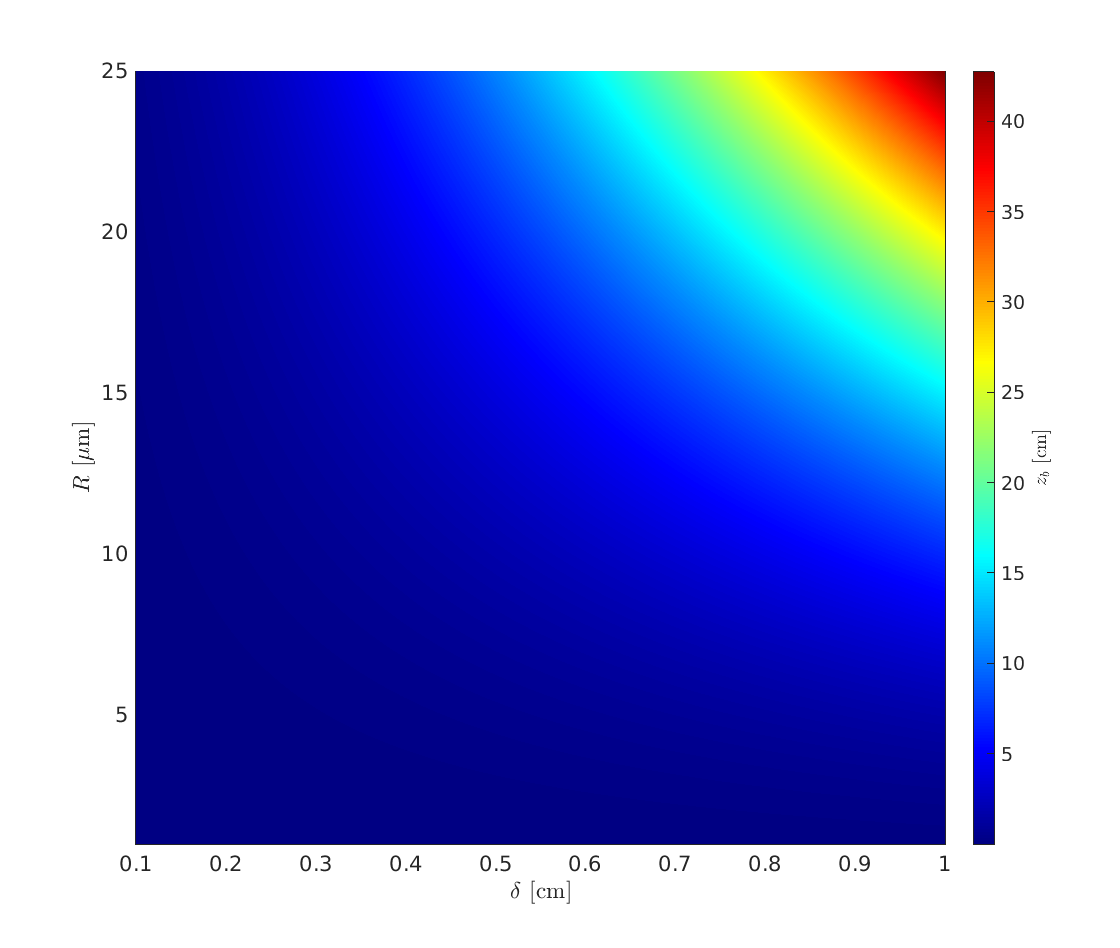
\includegraphics[width=30pc]{gfx/z_b_vs_delta_R.png}
\caption{Equillibrium position $z_b$ versus vortex core size $\delta$ and particle radius $R$. Plot variables' ranges correspond to cloud-like conditions.}
\label{fig:ch3_0}
\end{figure*}

Eq. \ref{ch2:03c} can be integrated with arbitrary constants $C_1$ and $C_2$ leading to the following general solution:
\begin{equation}
z^+(t)=C_1 \exp{\lambda_1 t^+}+C_2 \exp{\lambda_2 t^+}+z^+_b
\label{ch3:eq05}
\end{equation}
so $z^+(t)$ indeed depends exponentially on time.
By setting the initial conditions to $z^+(0)=z^+_0$, $\dot{z}(0)=w_0$ one obtains the following specific solution:
\begin{align}
\frac{z^+(t^+)-z^+_b}{z^+_0-z^+_b}=\frac{1}{\lambda_1-\lambda_2} \left[ \lambda_1 \exp{\lambda_2 t^+}-\lambda_2 \exp{\lambda_1 t^+} + \frac{w^+_0}{z^+_0-z^+_b}\left( \exp{\lambda_1 t^+}- \exp{\lambda_2 t^+}\right)\right] \\
\lambda_{1/2}=\left( \mp \sqrt{1+4 A St}-1\right)/2 St
\label{ch3:eq06}
\end{align}
This equation describes particle motion along the axis, by expressing the evolution of particle distance from equilibrium point with respect to its initial distance from the equilibrium point. In order to give a sense of this solution, it was rewritten using the newly defined dimensionless $k$ parameter:
\begin{equation}
k=(1+4 A St)^{-\frac{1}{2}}=(1+2\tau_p \gamma)^{-\frac{1}{2}}
\end{equation}
where $k \in (0,1)$, and dimensionalized:
\begin{equation}
\frac{z(t)-z_b}{z_0-z_b}=
\left[\frac{1}{2}\left(1-k\right)-k\frac{\tau_p w_0}{z_0-z_b}\right] e^{\frac{-t}{2 \tau_p}(k^{-1}+1)}+
\left[\frac{1}{2}\left(1+k\right)+k\frac{\tau_p w_0}{z_0-z_b} \right] e^{\frac{t}{2 \tau_p}(k^{-1}-1)}.
\label{ch3:eq08}
\end{equation}
One can see that the first term in \ref{ch3:eq08} is leading for small times, especially when the initial velocity is nonzero. In longer times the second term is a leading term.\\
As has already been argued in the introduction, the Burgers vortex is a good approximation for a long-lasting vortex only locally in space and time in turbulent flow. Therefore, the motion of particles in a vortex which has finite size and lifetime should be considered. For this reason further discussion of particle motion along the axis is devoted to the estimation of what is here defined as \emph{exit time} $\tau_{ex}$:\marginpar{exit time} the time at which a particle starting at position $z(t=0)=z_0$, with zero initial velocity $\dot{z}(t=0)=0$, reaches an arbitrary finite domain border $\pm Z$.\\
First, the Eq. \ref{ch3:eq08} for the initial velocity set to zero, $w_0=0$, simplifies to:
\begin{equation}
\frac{z(t)-z_b}{z_0-z_b}=\frac{1}{2}\left(1-k\right) e^{\frac{-t}{2 \tau_p}(k^{-1}+1)}+\frac{1}{2}\left(1+k\right) e^{\frac{t}{\tau_p}(k^{-1}-1)}
\label{ch3:eq11}
\end{equation}
In this case, the direction of motion depends on the relative position of $z_0$ and $z_b$ only. This thesis assumes that particles are significantly smaller then vortex size: $R<<\delta$, and thus $\tau_p \gamma <<1$. In large times $t>>\tau_p$ this assumption allows to approximate Eq.\ref{ch3:eq11} to:
\begin{equation}
\frac{z(t)-z_b}{z_0-z_b}=e^{\frac{t}{\tau_z}}
\label{ch3:eq12}
\end{equation}
where $\tau_z$ is the characteristic time of the motion along vortex axis:
\begin{equation}
\tau_z=\frac{2}{k^{-1}-1} \tau_p=\frac{2}{\sqrt{1+2\tau_p \gamma}-1} \tau_p
\label{ch3:eq09}
\end{equation}
According to small particles assumption, $\tau_z$ can be approximated as well:
\begin{equation}
\tau_z\approx \frac{2 \tau_p}{1+ 2\tau_p \gamma/2 -1}=2\gamma^{-1}=\nu^{-1}\delta^2.
\label{ch3:eq10}
\end{equation}

\begin{figure*}
\centering
\noindent 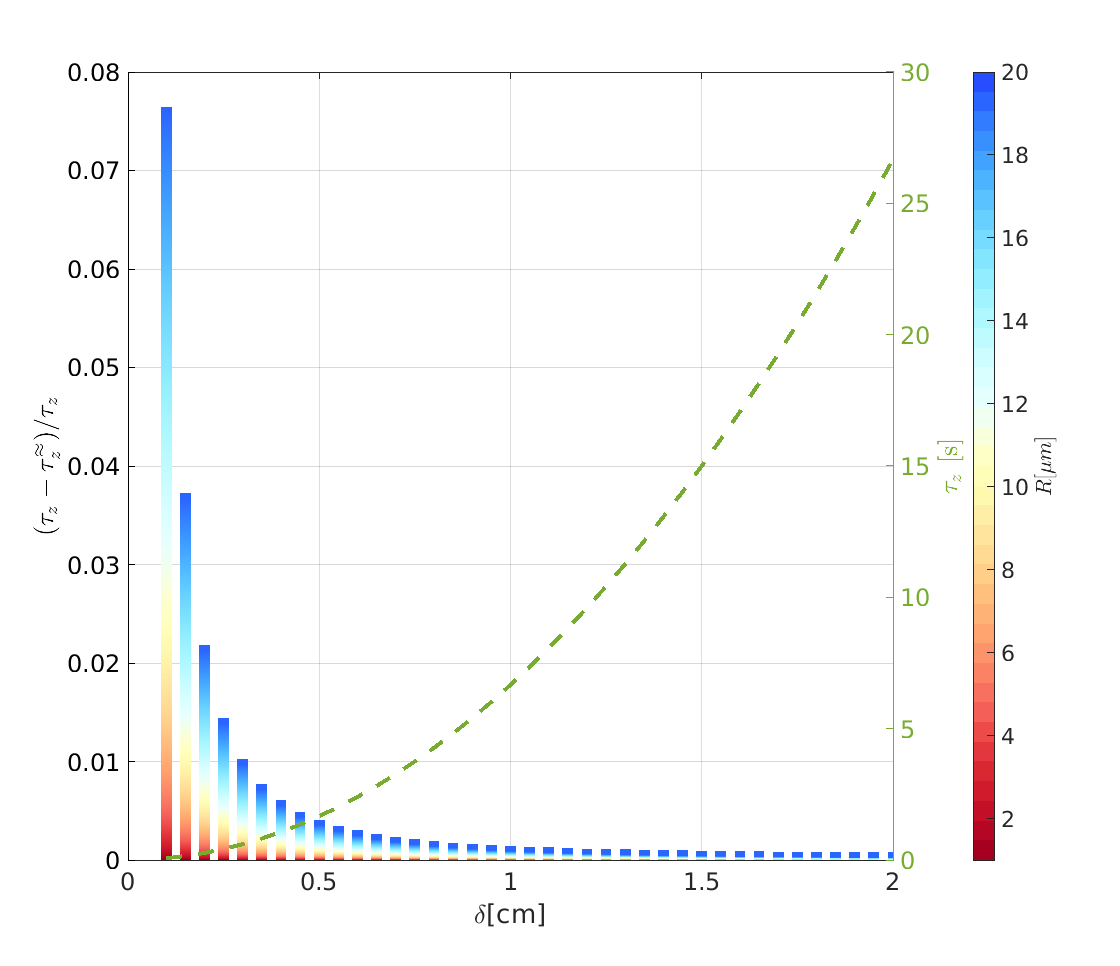
\includegraphics[width=30pc]{gfx/tau_z_error_tau_z_vs_delta.png}
\caption{Characteristic time of the motion along vortex axis $\tau_z$ (green line, right y-axis) versus vortex core size $\delta$ and its relative error (left y-axis, bar chart) versus $\delta$ and particle radius $R$. Colorscale indicates dependence on $R$. Plot variables' ranges correspond to cloud-like conditions.}
\label{fig:ch3_1}
\end{figure*}

Figure \ref{fig:ch3_1} presents $\tau_z$ relative arror (accurate value from Eq.\ref{ch3:eq09} minus approximated value from Eq.\ref{ch3:eq10} divided by the acurate value) with respect to $\delta$ (on X-axis) and $R$ (color). We see that for cloud-like variables' ranges the approximation is fully justified. What is interesting is that the approximated $\tau_z$ does not depend on particle size, so it is the same for all the particles in polydisperse dispersion. It is also easy to notice that in cloud-like conditions particle response time is always significantly smaller then characteristic time of motion along axis $\tau_z>>\tau_p$. For example when the vortex core size $\delta$ is 1~cm, then $\tau_z$ is approximately 6.7~s, and for 0.5cm it is approximately 1.6~s.\\
The simplified equation of motion, Eq.{ch3:eq12}, must be solved in order to estimate the exit time:
\begin{equation}
\frac{sign(z_0-z_b)Z-z_b}{z_0-z_b}=e^{\frac{\tau_{ex}}{\tau_z}}
\label{ch3:eq07}
\end{equation}
so there is:
\begin{equation}
\tau_{ex}=\tau_z \log\left(\frac{sign(z_0-z_b)Z-z_b}{z_0-z_b} \right)
\label{ch3:eq12b}
\end{equation}
The function under the logaritm is denoted as $L(Z,z_0;z_b)$ and further:
\begin{equation}
L(Z,z_0;z_b)=\frac{Z-sign(z_0-z_b)z_b}{|z_0-z_b|}=\frac{Z/z_b-sign(z_0-z_b)}{|z_0/z_b-1|}=
\frac{\overbrace{Z/z_b}^{Z^\ast}-sign(z_0/z_b-1)}{|\underbrace{z_0/z_b}_{z_0^\ast}-1|}.
\label{ch3:eq13}
\end{equation}
Then the estimated exit time:
\begin{align}
\tau_{ex}(Z^\ast,z_0^\ast; \tau_z)\approx \tau_z \log\left(L(Z^\ast,z_0^\ast)\right)\\
L(Z^\ast,z_0^\ast)= \frac{Z^\ast-sign(z_0^\ast-1)}{|z_0^\ast-1|}\\
\label{ch3:eq14}
\end{align}
where $Z^\ast \in (1,\infty), \ z_0^\ast \in [-Z^\ast,1)\cup (1,Z^\ast]$. For $z_0^\ast=1$ (when $z_0=z_b$) the estimation gives $\tau_{ex}=\infty$, so it agrees with the fact, that $z_b$ is an unstable equillibrium point.

\begin{figure*}
\centering
\noindent 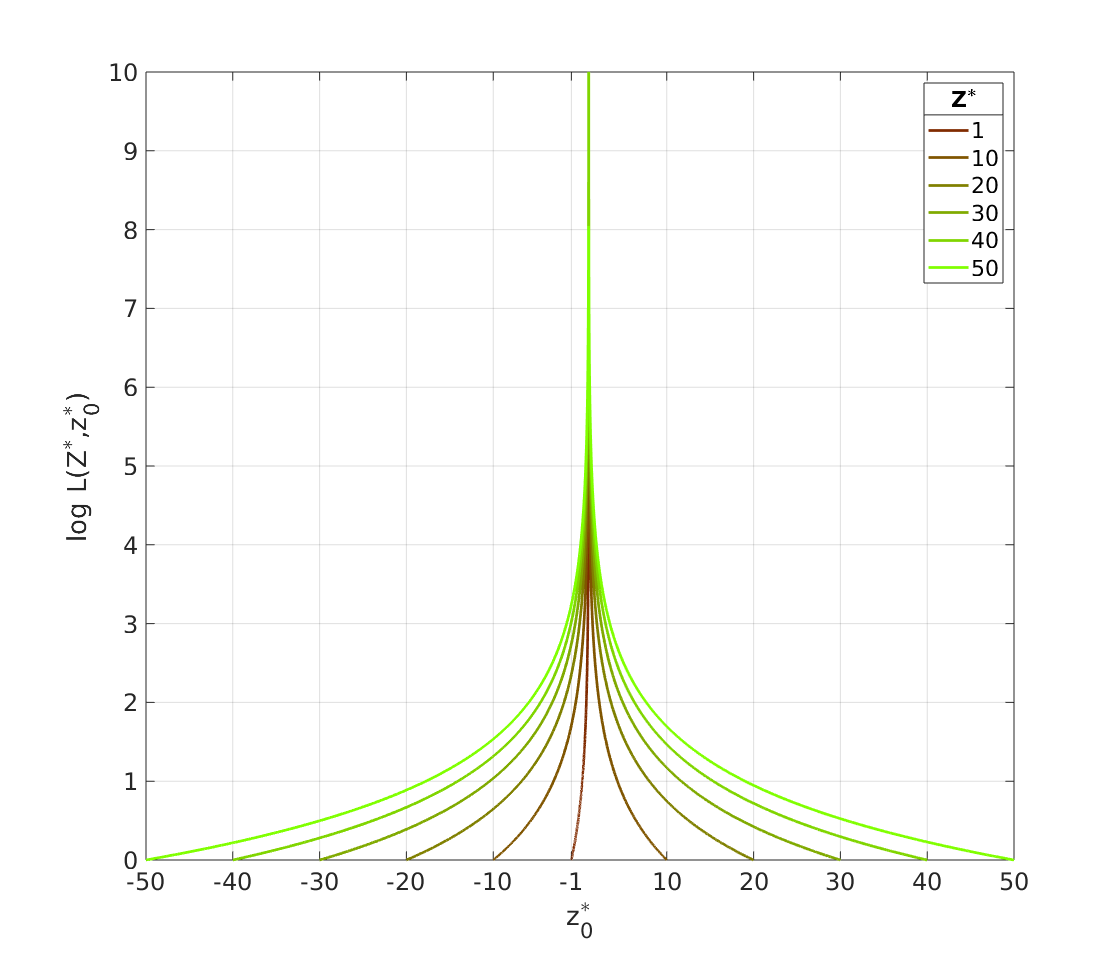
\includegraphics[width=30pc]{gfx/Z_log_factor_plot.png}
\caption{Logarithmic factor $logL$ (in $\tau_{ex}$) vs. $z^*_0$ - ratio of initial position and equillibrium position. Line color is scaled by $Z*$ values which refer to different ratios of vortex half-length and equillibrium position.}
\label{fig:ch3_2}
\end{figure*}

The logarithmic factor in $\tau_{ex}$ is depicted in Fig. \ref{fig:ch3_2}. It depends on domain half-length $Z$ and initial position $z_0$ ratios to $z_b$. It is hard to draw any direct conlusions for single particle exit time on the basis of Fig.\ref{fig:ch3_2} alone. However there is an interesting feature when thinking about the collection of particles in the vortex. Namely, the mean value of logarithmic factor over $z_0^\ast$ (over all initial positions) equals one for every $Z^\ast$ (for every vortex half-length):
\begin{equation}
\langle log\ L(Z^\ast,z_0^\ast)\rangle_{z_0^\ast}=\frac{1}{2 Z^\ast}\int_{-Z^\ast}^{Z^\ast}log\ L(Z^\ast,z_0^\ast)dz_0^\ast=1
\label{ch3:eq15}
\end{equation}
This means that independently of vortex length, when dealing with uniformly distributed set of particles, the logarithmic factor does not have influence on mean exit time.

\section{Motion in the plane perpendicular to vortex axis}

The trajectories determined in 2D space by Eq.\ref{ch2:eq03a}-\ref{ch2:eq03c} have several different attractors. The exact choice depends on the system parameters. Presence of gravity force distinguishes two basic cases. There are presented below.
%The analysis of single droplet motion in projection on a plane $(r,\varphi)$ perpendicular to the vortex axis was conducted by \citet{Marcu1995} and is summarized below.

\subsection{Without gravity (vertical vortex)}
The system without gravity force in 2D space is equal to the system in which gravity is parallel to the vortex axis ($\theta=0$). It comes down to the fact that sedimentation parameter $S_v$ is zero. In this case the nondimensional equations of motion are:
\begin{equation}
\left\{\begin{array}{l}
\ddot{r^+}-r^+\dot{\varphi^+}^2=-St^{-1}\left(A r^++\dot{r^+}\right) \\
2\dot{r^+}\dot{\varphi^+}+r^+\ddot{\varphi^+}=St^{-1}\left(\frac{1}{2 \pi r^+}(1-e^{-\frac{r^{+ 2}}{2}})-r^+\dot{\varphi^+}\right)\\
\end{array}.\right.
\label{ch3:eq16}
\end{equation}
and the system posses axial symmetry. This set of equations depends on two parameters only: $St/A$ and $St$. The attractors: an equillibrium point positioned on the vortex axis $r^+=0$ or a circular orbit of radius $r^+_{orb}$ (defined later), inherit the axial symmetry. The system changes according to Hopf bifurcation scheme when $\alpha=16 \pi^2-St/A$ is a bifurcation parameter. This translates to the fact, that if:
\begin{equation}
St \geq St_{cr}(A) \equiv 16 \pi^2 A,
\label{ch3:eq17}
\end{equation}
the only attractor, the equillibrium point at the axis, is a stable focus ($\alpha \leq 0$). In the opposite case $St < St_{cr}$, the equilibrium point is an unstable focus, accompanied by a stable periodic cicular orbit ($\alpha>0$). Particle trajectories around such attractors are presented schematically in Fig. \ref{fig:ch2_04}. Having established the existence of attractors, their impact on particle kinematics is studied.\\

\begin{figure*}
\centering
\noindent 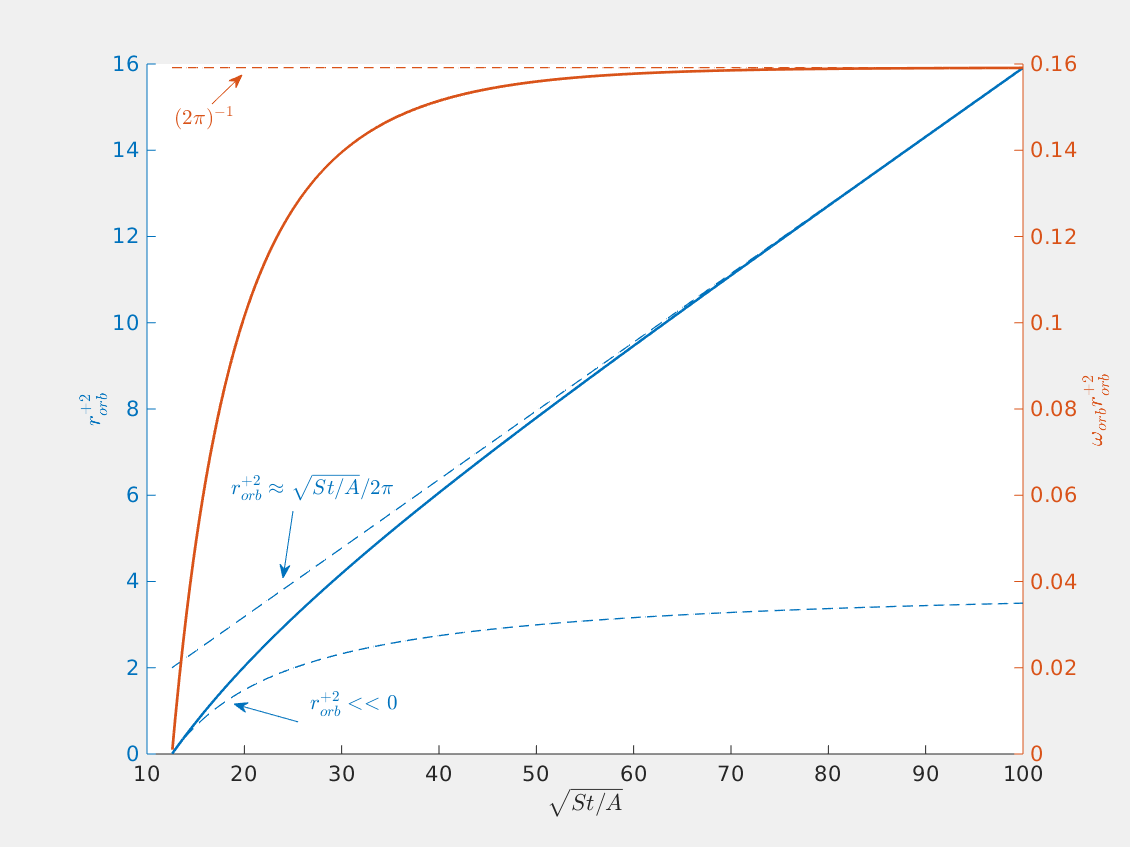
\includegraphics[width=30pc]{gfx/r0_2_sqrt_St_A_omega_r0_2.png}
\caption{Particle stable orbit radius $r^+_{orb}$ square (left y-axis) and orbit nondimensional angular momentum (right y-axis) with respect to parameter $\sqrt{St/A}$. Dashed lines represent asymptotic relations.}
\label{fig:ch3_3}
\end{figure*}

\subsubsection{Stable periodic orbit}

The first type of trajectory that is analysed is the particle moving on stable periodic orbit. The radius of the periodic orbit, denoted as $r^+_{orb}$, satisfies the equation:
\begin{equation}
 \left[1-\exp\left( -r^{+ 2}/2 \right) \right]/2 \pi r^{+ 2}=\sqrt{A/St}, 
\label{ch3:eq18}
\end{equation}
which depends uniquely on $St/A$. Numerical solution of this equation for an arbitrary parameter range, starting at $\sqrt{St_{cr}/A}$, is presented in Fig. \ref{fig:ch3_3}. This plot suggest that we can distinguish two asymptotic limits in the solution. For small orbit radius, $r^+_{orb}<<1$, it is possible to approximate leftside of Eq.\ref{ch3:eq18} by developing Taylor series around zero and get:
\begin{equation}
 \left[1-\exp\left( -r^{+ 2}/2 \right) \right]/2 \pi r^{+ 2}\approx \left(\frac{1}{2}-\frac{r^{+ 2}}{8}+O(r^{+ 4})\right)/2 \pi
\label{ch3:eq18a}
\end{equation}
which then gives the relation shown in Fig.\ref{fig:ch3_3} by curved dashed blue line. In the limit of large orbit radius there is:
\begin{equation}
 \left[1-\exp\left( -r^{+ 2}/2 \right) \right]/2 \pi r^{+ 2}\approx \left(r^{+ -2}+O(r^{+ -4})\right) /2 \pi
\label{ch3:eq18b}
\end{equation}
which leads to the approximation:
\begin{equation}
r^+_{orb} \approx \frac{1}{2\pi} \sqrt{\frac{St}{A}}
\label{ch3:eq18c}
\end{equation}
shown in Fig.\ref{fig:ch3_3} as straight dashed blue line.
The second conclusion based on the solution to equation \ref{ch3:eq18} is that nondimensional angular velocity at circular periodic orbit is: $\omega^{+}_{orb}=\sqrt{A/St}$, or in other words, particle rotation time $\tau^+_{orb}=\sqrt{St/A}$. What is interesting, particle angular momentum $\omega^{+} r^{+ 2}$ on circular orbit (orange line plot in Fig. \ref{fig:ch3_3}, right Y-axis) in large radius limit is approximately constant in time and independent of particle size, equal to $(2 \pi)^{-1}$. \\
A cloud-like view at the periodic orbit issue is considered below. Periodic orbit existence condition from Eq.\ref{ch3:eq17} is reformulated to:
\begin{equation}
R \geq R_{cr}(A,\delta)=12 \pi \sqrt{\frac{\rho_a}{2\rho_p}}\  A \delta.
\label{ch3:eq19}
\end{equation}
The numerical solution presented in Fig.\ref{fig:ch3_3} are now shown in the Fig. \ref{fig:ch3_3a} in dimensional form, where vortex core size is chosen arbitrarly: $\delta=0.5~cm$. In this parameters' range, the particle orbit radius is of the order of vortex core size. One can see, that in the large orbit limit, from Eq.\ref {ch3:eq18c} there is:
\begin{equation}
r_{orb}\propto R^{1/2} \delta^{1/2} A^{-1/2}
\label{ch3:eq19b}
\end{equation}

\begin{figure*}
\centering
\noindent 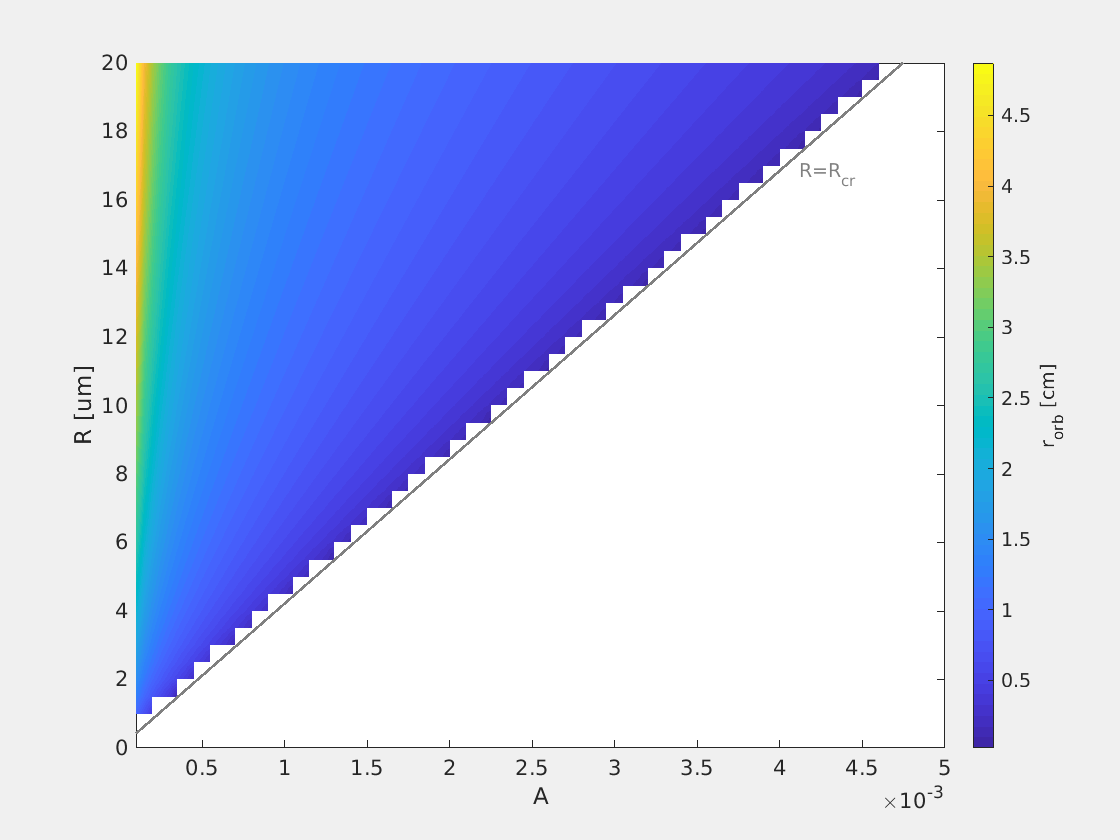
\includegraphics[width=30pc]{gfx/orbit_vs_R_A_delta05cm.png}
\caption{Particle stable orbit radius $r_{orb}$ dependence on  particle radius $R$ and vortex strain parameter $A$ for cloud-like parameter ranges and vortex core size $\delta=0.5~cm$. Black line represents stable orbit existence condition.}
\label{fig:ch3_3a}
\end{figure*}

It is interesting to notice that the dimensional angular velocity $\omega_{orb}$ is independent of $A$. It is in fact inversly proportional to particle radius $R$ and vortex core size $\delta$:
\begin{equation}
\omega_{orb}=\sqrt{A/St} \tau_f^{-1}=\delta^{-1} \sqrt{\nu \tau_p^{-1}}=\sqrt{\gamma(2\tau_p)^{-1}}=3 \nu \sqrt{\rho_a /2 \rho_p} (R \delta)^{-1} \propto (R \delta)^{-1}.
\label{ch3:eq20}
\end{equation}

Fig.\ref{fig:ch3_3b} presents cloud-like values of angular velocity $\omega_{orb}$. It is itself independent of $A$, but it is the periodic orbit existence condition that depends on $A$. The existence condition is presented in Fig.\ref{fig:ch3_3b} by  $R=R_{cr}(A)$ plots. For a given $A$ periodic orbits exist in  $R>R_{cr}(A)$ area.

\begin{figure*}
\centering
\noindent 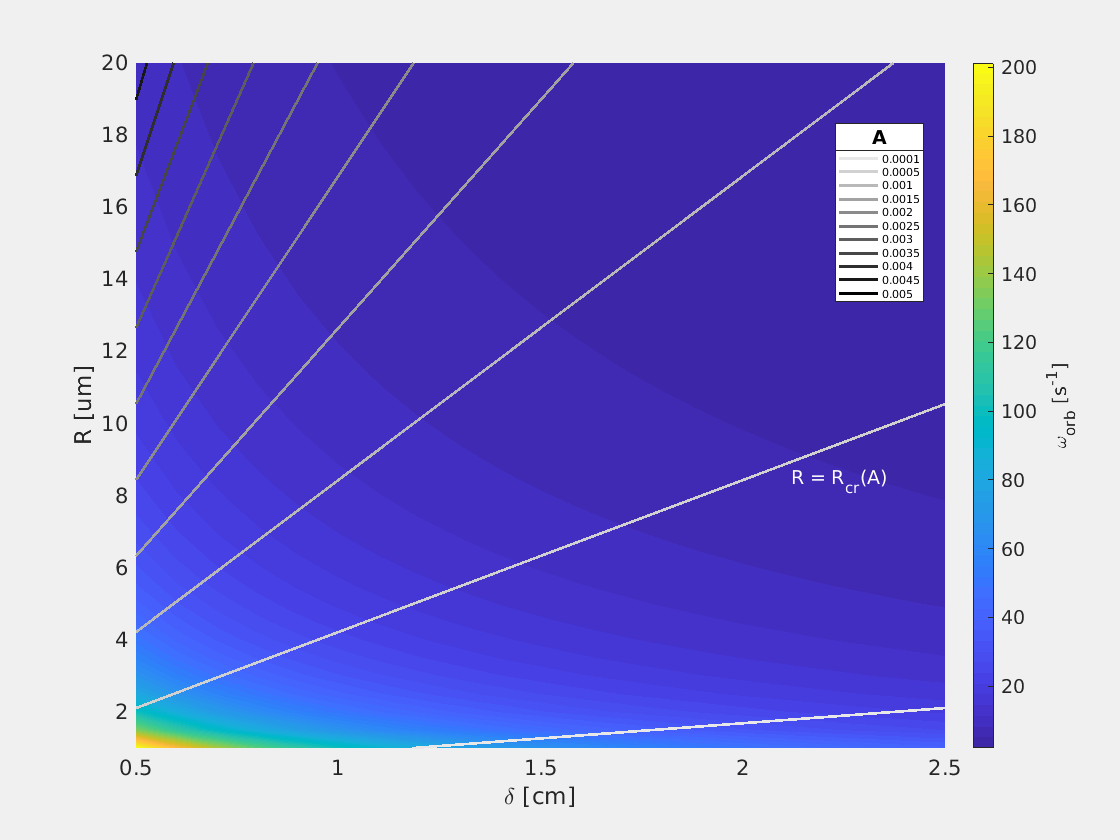
\includegraphics[width=30pc]{gfx/orbit_vel_vs_R_and_delta.png}
\caption{Particle stable orbit angular velocity $\omega_{orb}$ dependence on particle radius $R$ and vortex core radius $\delta$ for cloud-like parameter ranges.}
\label{fig:ch3_3b}
\end{figure*}

Particle rotation time being an inverse of angular velocity is proportional to vortex core radius and particle radius:
\begin{equation}
\tau_{orb}=\sqrt{2 \tau_p \gamma^{-1}} \propto R \delta.
\label{ch3:eq21}
\end{equation}

The previously established assumption of small particles  i.e. $\tau_p<<\gamma^{-1}$ leads to the conclusion that $\tau_{orb}<<\gamma^{-1}$ as well. More on the timescales of motion can be found later in the text.\\
Having identified system attractors and their basic features, their realistic impact on particle kinematic is studied. The probability that a particle founds itself in phase space exactly in the equilibrium point or on periodic orbit is low. More probable is that it is positioned somewhere else and is pulled towards its attractor/s. That fact is the motivation for the detailed study of particles approaching their attractors conducted below.\\

\subsubsection{Stable focus or stable periodic orbit attraction}
I analyze the scales of motion and features of the particle trajectory starting at arbitrary position and approaching its attractor (stable focus at the axis or circular orbit). For the sake of simplicity, the starting radial positions selected for analysis are the only spatial scales distinguished in the equations. That means: the position at the axis $r^+(0)=0$ and at $r^+(0)=r_s$. The motion of a particle defined in this way is called here a "docking process".\marginpar{docking process} Time at which the docking process occures is consequently called docking time and noted $t^+_{doc}$. In short, for the purposes of further analysis, I distinguish two types of processes:
\begin{itemize}
\item in-orbit docking: $r^+(0)=0$, $\dot{r^+}(0)=u_r^+(0)$, particle is attracted by its periodic orbit $r^+_{orb}$
\item axis docking: $r^+(0)=r_s$, $\dot{r^+}(0)=u_r^+(r_s)$ particle is attracted by a point on vortex axis $r^+=0$.
\end{itemize}
Due to the fact, that the particle approaches its destined radial position asymptotically, numerical simulation of the docking process was defined between points in the phase space indicated in the Table \ref{tab:ch3_1}.

\begin{table}
\small
\tabcolsep=0.2cm
\centering
\caption{Initial ($t^+=0$) and final ($t^+=t^+_{doc}$) particle state in numerical simulations of docking processes. $\sigma$ is an arbitrary small parameter.}
\centering
\begin{tabular}{|l||c|c|c|}
\hline 
docking& $r^+(0)$ & $\dot{r^+}(0)$ & $r^+(t^+_{doc})$\\
\hline \hline
in-orbit & $\sigma$ & $u^+_r(\sigma)$ & $r^+_{orb}-\sigma$\\
\hline
axis & $r_s-\sigma$ & $u_r^+(r_s-\sigma)$ & $\sigma$\\
\hline
\end{tabular}
\label{tab:ch3_1}
\end{table}

The choice of small $\sigma$ parameter will be elaborated on later.\\

\begin{figure*}
\centering
\noindent 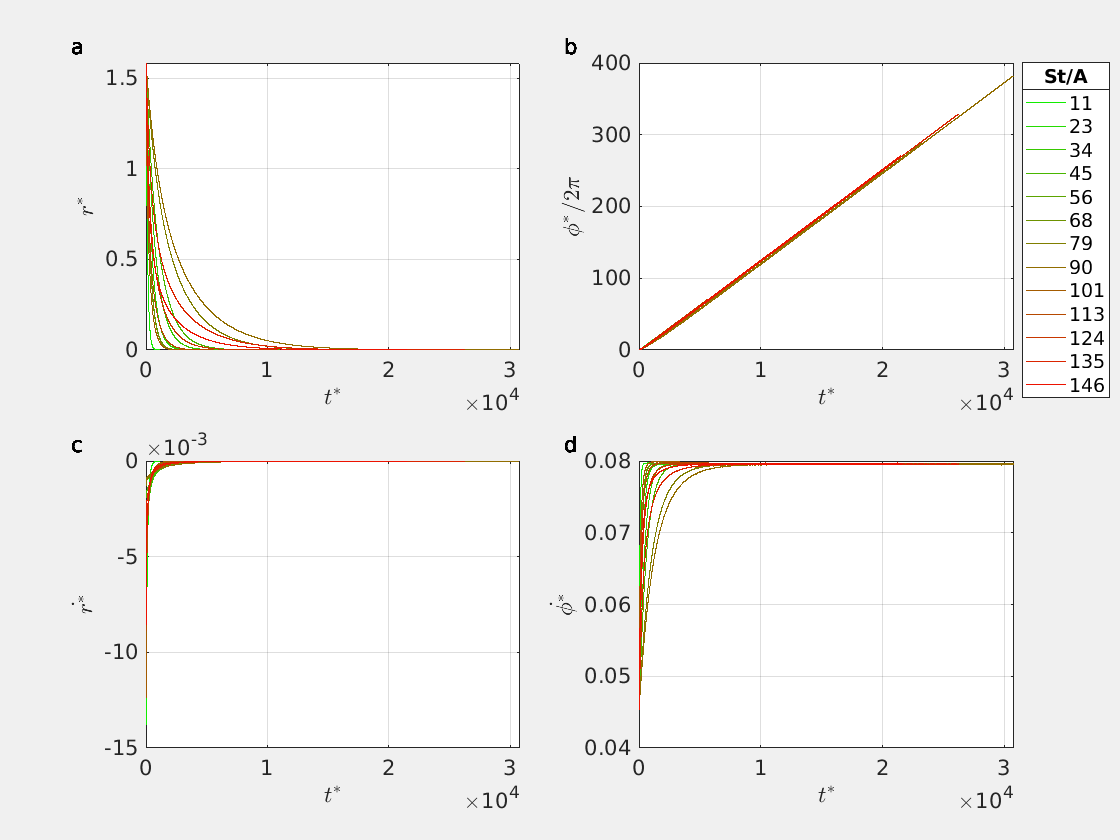
\includegraphics[width=30pc]{gfx/point_docking_vel_traj_in_time_noscal.png}
\caption{Tracking of a particle while docking on axis, for  $\sigma=10^{-4}$. Line color corresponds to $St/A$ value, line color intensity to different $St$ and $A$ representations. Upper panel- radial coordinate, middle panel - radial velocity, lower panel - angular velocity.}
\label{fig:ch3_42}
\end{figure*}

\begin{figure*}
\centering
\noindent 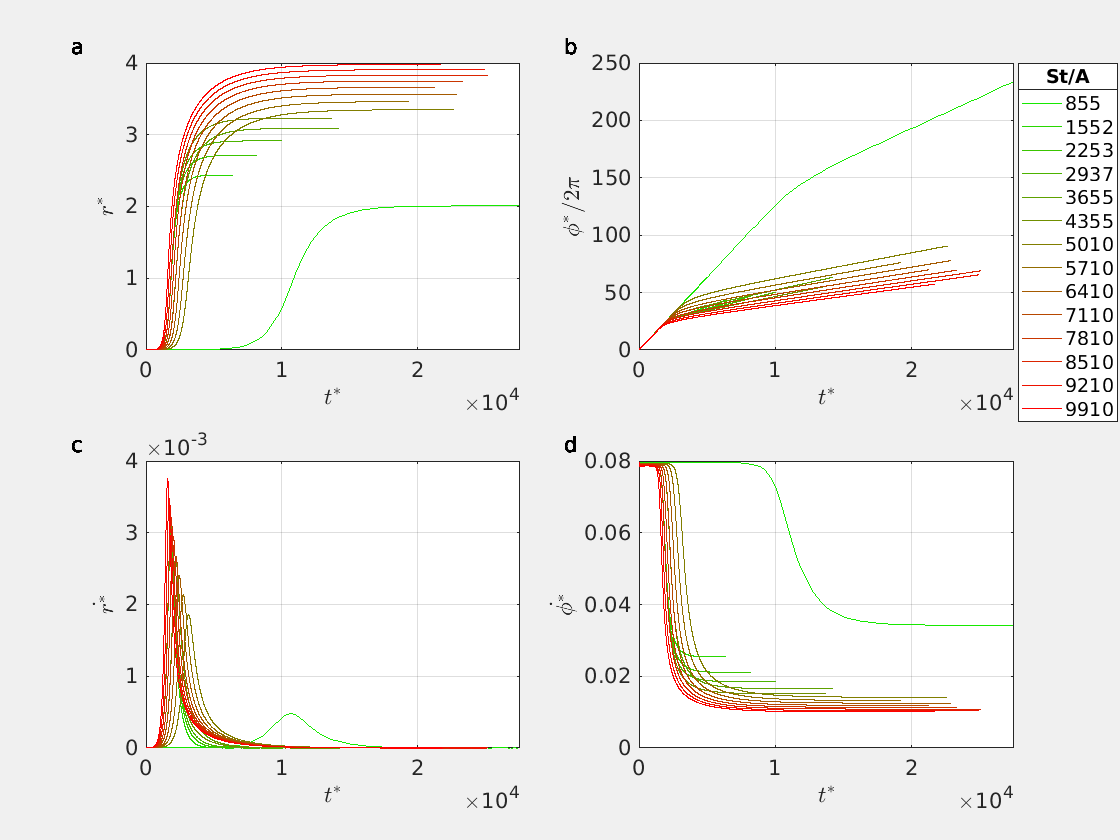
\includegraphics[width=30pc]{gfx/orbit_docking_vel_traj_in_time_noscal.png}
\caption{Tracking of a particle while docking in orbit, for $\sigma=10^{-4}$. Line color corresponds to $St/A$ value, line color intensity to different $St$ and $A$ representations. Upper panel- radial coordinate, middle panel - radial velocity, lower panel - angular velocity.}
\label{fig:ch3_41}
\end{figure*}

Figure~\ref{fig:ch3_42} and Fig.~\ref{fig:ch3_41} show tracking particles wich undergoes docking process, on axis and in-orbit respectively. Three panels show radial position, radial velocity and angular velocity of particles. Each line represents a particle with different $St$ and $A$ parameters. Line color corresponds to $St/A$ value, line color intensity to different $St$ and $A$ representations of the same $St/A$ value. From Fig.~\ref{fig:ch3_42} it is hard to see any rule on parameter dependence. All the particles tend to have the same angular velocity when they dock on the axis, the radial velocity towards the axis dimnish in time in a kind of exponential manner. The ratio at which it happens depends on both $St$ and $A$, the same is for $t^+_{doc}$. In Fig.~\ref{fig:ch3_42} one can notice, that particles has the same angular velocity at the start and it decreases to a value determined by $St/A$ only. The same time the radial velocity rises and falls again to zero almost symmetrically in time, when the particle reaches its orbit at $r^+_{orb}$. 

\begin{figure*}
\centering
\noindent 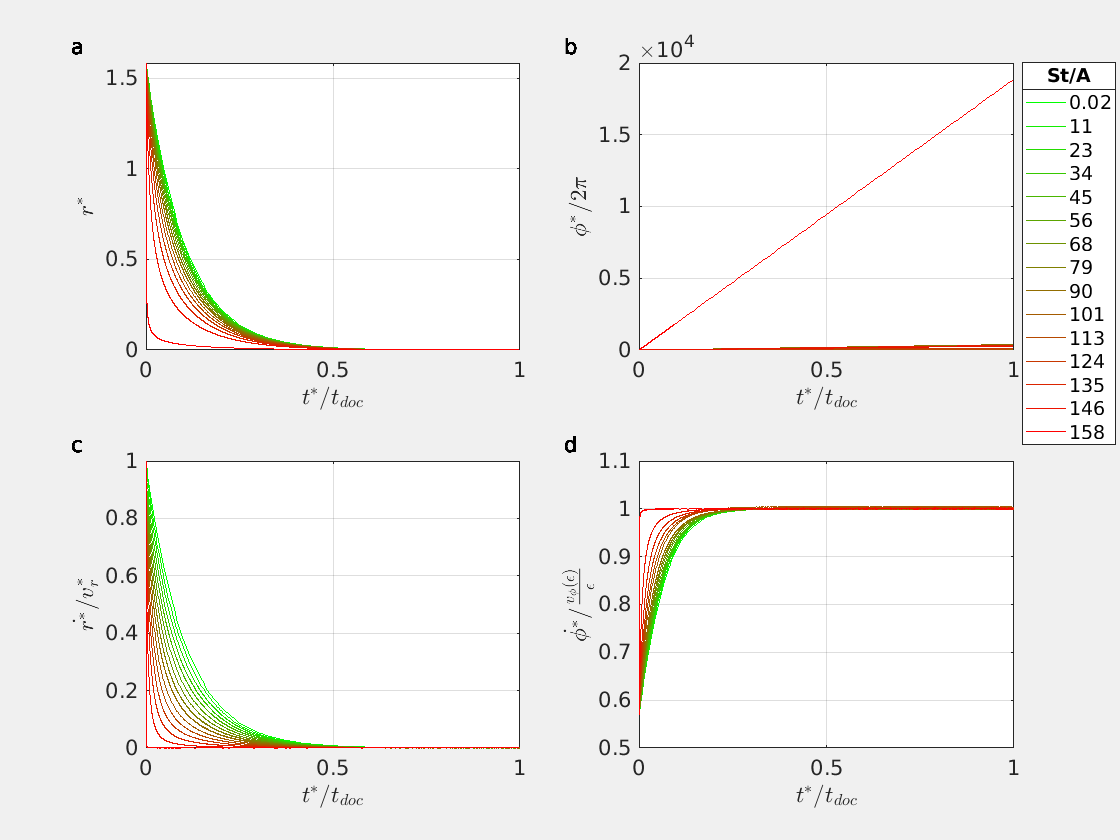
\includegraphics[width=30pc]{gfx/point_docking_vel_traj_in_time_scal.png}
\caption{Same as in Fig. \ref{fig:ch3_42}, but X-axis is scaled separately for each trajectory by a docking time. On Y-axes, the radial velocity is scaled by the fluid velocity at the starting point $u_r(r_s)$, angular velocity is scaled by the fluid angular velocity at the final position $\sigma$, so $u_{\varphi}(\sigma)/\sigma$.}
\label{fig:ch3_44}
\end{figure*}

\begin{figure*}
\centering
\noindent 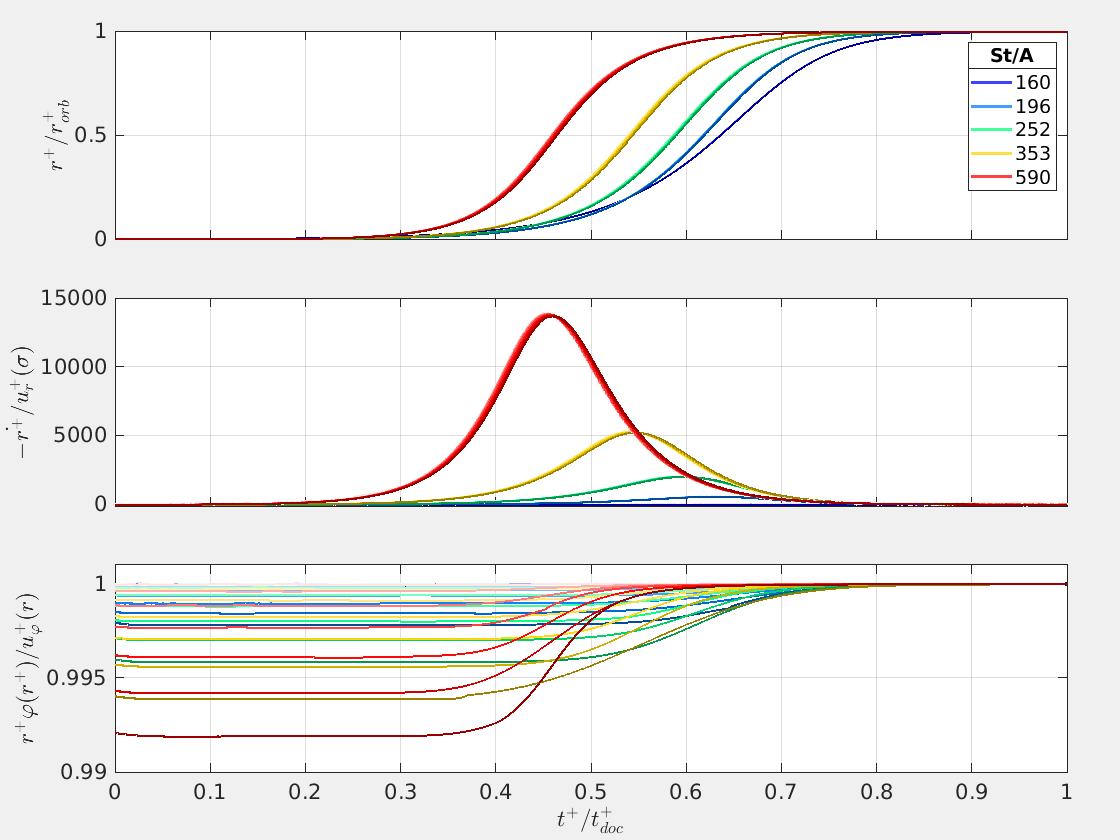
\includegraphics[width=30pc]{gfx/orbit_docking_vel_traj_in_time_scal.png}
\caption{Same as in Fig. \ref{fig:ch3_41}, but X-axis is scaled separately for each trajectory by docking time. On Y-axes, radial position is scaled by circular orbit radius, radial velocity is scaled by the opposite of fluid velocity at the starting point $-u_r(\sigma)$, angular velocity is scaled by the fluid angular velocity  $u_{\varphi}(r^+)/r^+$.}
\label{fig:ch3_43}
\end{figure*}

Figure~\ref{fig:ch3_44} and Fig.~\ref{fig:ch3_43} represent the same data, but rescaled. X-axis is scaled separately for each trajectory by docking time. In Fig.~\ref{fig:ch3_44}, on Y-axes, the radial velocity is scaled by the fluid velocity at the starting point $u_r(r_s)$, angular velocity is scaled by the fluid angular velocity at the final position $\sigma$, so $u_{\varphi}(\sigma)/\sigma$. In Fig.~\ref{fig:ch3_43},
on Y-axes, radial position is scaled by circular orbit radius, radial velocity is scaled by the opposite of fluid velocity at the starting point $-u_r(\sigma)$, angular velocity is scaled by the fluid angular velocity  $u_{\varphi}(r^+)/r^+$. By doing so, one can obtain trajectories that depend almost only on $St/A$ parameter - lines of the same color, but different intensity, converge. The greatest difference is seen in particle angular velocity response to fluid, which is caused by different $St$. Fig.\ref{fig:ch3_43} reveals that when the particle is docking in-orbit, it first followes the fluid motion around the axis, with radial velocity close to zero. With rotational velocity, the centrifugal force starts acting on it and causes a rapid increase in radial speed in the direction away from the vortex axis. Increasing distance from the axis in turn results in a steep decrease of the angular velocity, and further the decrease of the radial velocity. Then the particle approaches its periodic orbit: radial velocity goes to zero, rotational velocity goes to $\omega_{orb}$. The rate of these changes depends on the parameters of the model in a complex way. The attempt to find the approximate dependence is conducted below.\\



% tutaj o probie oszacowania ruchu dokowania na orbicie



Now lets look closer at the axis docking process. Figures \ref{fig:ch3_42} and \ref{fig:ch3_44} show that  the particle firstly move with radial velocity the same as fluid's velocity: $v^+_r(r_s-\sigma)$. Next the particle radial velocity decreases almost exponentially in time. When the time is scaled by docking time, $t^+/t^+_{doc}$, the rate of exponential decrease depends on $St/A$ parameter only. Angular velocity increases towards fluid velocity close to the axis, $v^+_{\varphi}(\sigma)/\sigma$, when particle is approching the axis.\\
\noindent The first glance at \ref{fig:ch3_42} and \ref{fig:ch3_44} leads to the observation that the radial motion (as for $r(t)$ and $\dot{r}(t)$) of the particle docking on the axis is close to exponential. Therefore, a simplified model of this process is proposed below and an attempt is made to estimate axis docking timescale $\tau^+_{d1}$.\\
Lets assume that in the axis docking process we have:
\begin{equation}
\left\{\begin{array}{l}
\dot{r}^+(t)=u_r^+(r_s-\sigma) \exp \frac{-t}{\tau^+_{d1}}, \\
r^+(0)=r_s-\sigma, \\
r^+(t_{doc})=\sigma 
\end{array}.\right.
\label{ch3:eq22}
\end{equation}
Then:
\begin{equation}
r^+(t^+)=r_s-\sigma+(r_s-\sigma)A\tau^+_{d1}\left(\exp\frac{-t^+}{\tau^+_{d1}}-1\right).
\label{ch3:eq23}
\end{equation}

The numerical simulations' results presented in Fig. \ref{fig:ch3_44} suggest that it is reasonable to assume: $t^+_{doc}/\tau^+_{d1}= h\left(St/A\right)$ where $h\left(St/A\right)$ is an unknown function of its single parameter. This assumption used in the relation for $t^+_{doc}$ based on Eq.\ref{ch3:eq22} gives:

\begin{equation}
r^+(t^+_{doc})=r_s-\sigma+(r_s-\sigma)A\tau^+_{d1} (\exp\left(-h\left(St/A\right)\right)-1)=\sigma
\label{ch3:eq24}
\end{equation}
and further:
\begin{equation}
\tau^+_{d1} \simeq \frac{r_s-2\sigma}{r_s-\sigma} \frac{1}{A} \left[1-\exp\left(-h\left(St/A\right)\right)\right]^{-1}
\label{ch3:eq25}
\end{equation}

This could suggest that first order approximation for point docking timescale is $\tau^+_{d1} \sim \ A^{-1}$. In order to numerically verify accuracy of this approximation, the relation proposed in Eq. \ref{ch3:eq22} was fitted to particle trajectories, with $\tau^+_{d1}$ serving as the fitting parameter. Fig. \ref{fig:ch3_45} presents the scatter plot of the fitting results times $A$. Point color represents Stokes number, point size refers to $A$. Mind, that the lower Y-axis limit is 1.

\begin{figure*}
\centering
\noindent 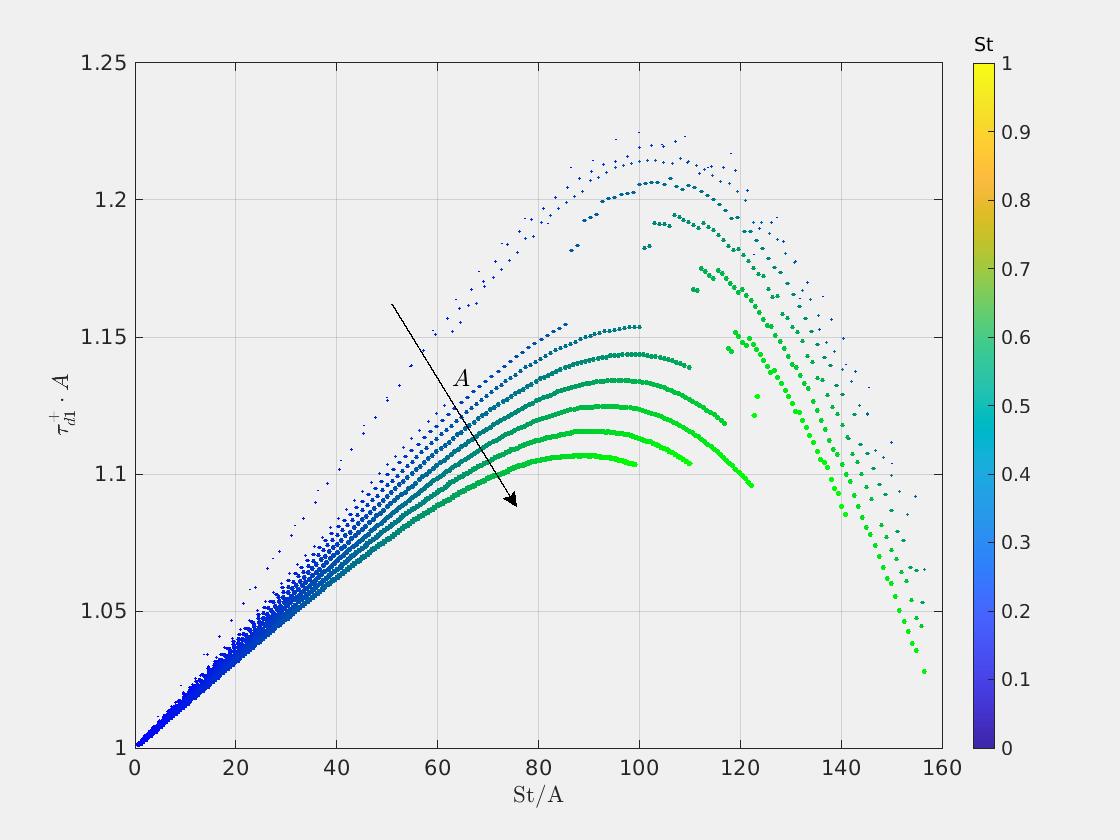
\includegraphics[width=30pc]{gfx/point_docking_taud1A_vs_St_A.png}
\caption{Results of fitting the relation proposed in Eq. \ref{ch3:eq22} to particle trajectories with the fitting parameter $\tau^+_{d1}$. For transparency Y axis shows fitting parameter times $A$. Point color represent Stokes number, point size - strain parameter $A$.}
\label{fig:ch3_45}
\end{figure*}
In Fig. \ref{fig:ch3_45} fitted values $\tau^+_{d1} \cdot A$ are close to one. This leads to the conclusion that axis docking timescale can be estimated by $A^{-1}$. Dimensional axis docking timescale is then:

\begin{equation}
\tau_{d1} \simeq A^{-1} \tau_f=2 \gamma^{-1}
\label{ch3:eq26}
\end{equation}
Estimated dimensional timescale $\tau_{d1}$ depends primarily on $\gamma^{-1}$. This is exactly the same as in the case of motion along vortex axis (see Eq.\ref{ch3:eq10}).\\




%in-orbit
fter scaling the time by $t^+_{doc}$ it can be noticed that the docking process depends mainly monotonically on the parameter $St/A$. When its value decreases towards $16 \pi^2$ the docking time $t^+_{doc}$ tends to infinity.
%%%
Another obsevation is that when $St/A$ increases towards the critical value $16 \pi^2$, the docking time $t^+_{doc}$  tends to infinity.
%%%%



Further the analysis of $t^+_{doc}$ for arbitrary parameter ranges was conducted. Figure \ref{fig:ch3_4} and \ref{fig:ch3_4x} present the results of $t^+_{doc}$ numerical calculation, with respect to $St$ and $A$ in 3D and 2D plots respectively. Blank spaces in the figures represent sets of parameters for which calculation was numerically expensive and hence the result was not included. Vertical axis in \ref{fig:ch3_4} and colorscale in both figures are logarithmic. Black line in Fig. \ref{fig:ch3_4x} respresents the $St=St_{cr}(A)$.

\begin{figure*}
\centering
\noindent 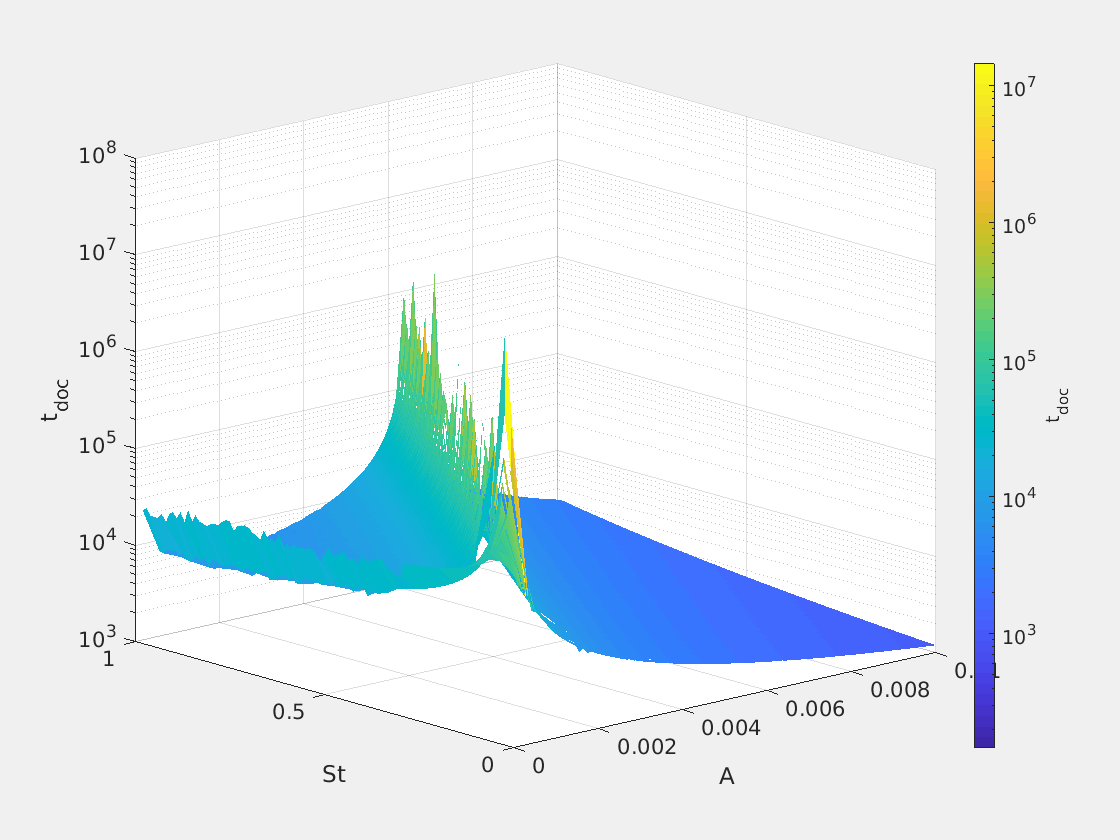
\includegraphics[width=30pc]{gfx/St_A_logt_exit_part_3D_eps000001_no_interp.png}
\caption{Docking time calculated numerically with respect to $St$ and $A$ for arbitrary variable ranges with $\sigma=10^{-5}$. Blank spaces represent lack of data, numerically too expensive.}
\label{fig:ch3_4}
\end{figure*}

\begin{figure*}
\centering
\noindent 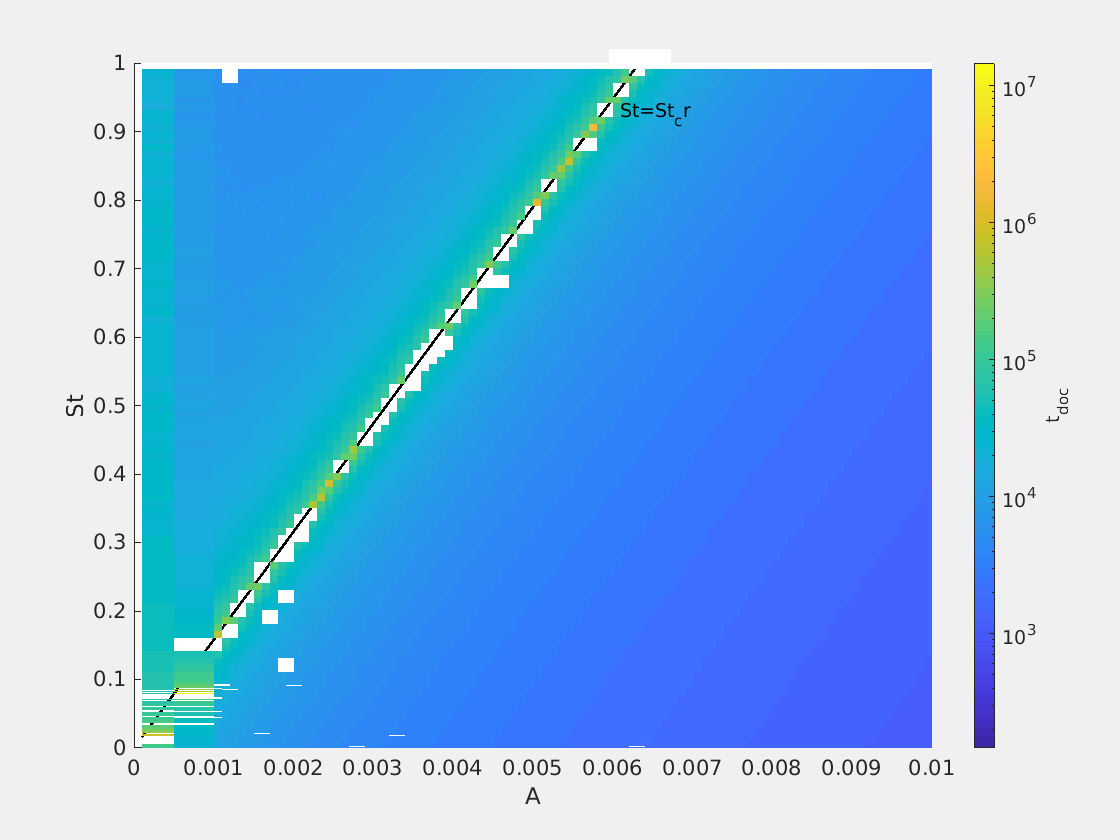
\includegraphics[width=30pc]{gfx/St_A_logt_exit_part_2D_eps000001_no_interp.png}
\caption{The same as in Fig. \ref{fig:ch3_4}, projection. Black line $St=St_{cr}(A)$ shows the stability boarder: particles to the left are attracted by periodic orbits, particles to the right by stable points on vortex axis.}
\label{fig:ch3_4x}
\end{figure*}

Fig. \ref{fig:ch3_4} and \ref{fig:ch3_4x} suggest some preliminary thoughts. First, defined in a twofold way the time $t_{doc}$ seems to have a physical sense: the values are of a similar order, and around the sharp boundary of two regimes: $St=St_{cr}(A)$ , they seem to tend towards infinity, what agrees with theroretical prediction. Secondly,\\
Tutaj jeszcze pozostaly ewentualnie do wrzucenia jakies wnioski z rysunkow?
\begin{itemize}
\item wyrazne szalone (log!) maksimum wokol $St=St_{cr}$, poniewaz sila dzialajaa na czastke jest malutka
\item Dla $St<St_cr$ glownym parametrem wydaje sie byc $St/A$ razy cos tam, bo linie sa prawie rownolegle
dla malych $A$ wzrost czasu prawie wylacznie ze zmniejszajacym sie $A$ - orbity sa tak daleko?
\end{itemize}


\begin{figure*}
\centering
\noindent 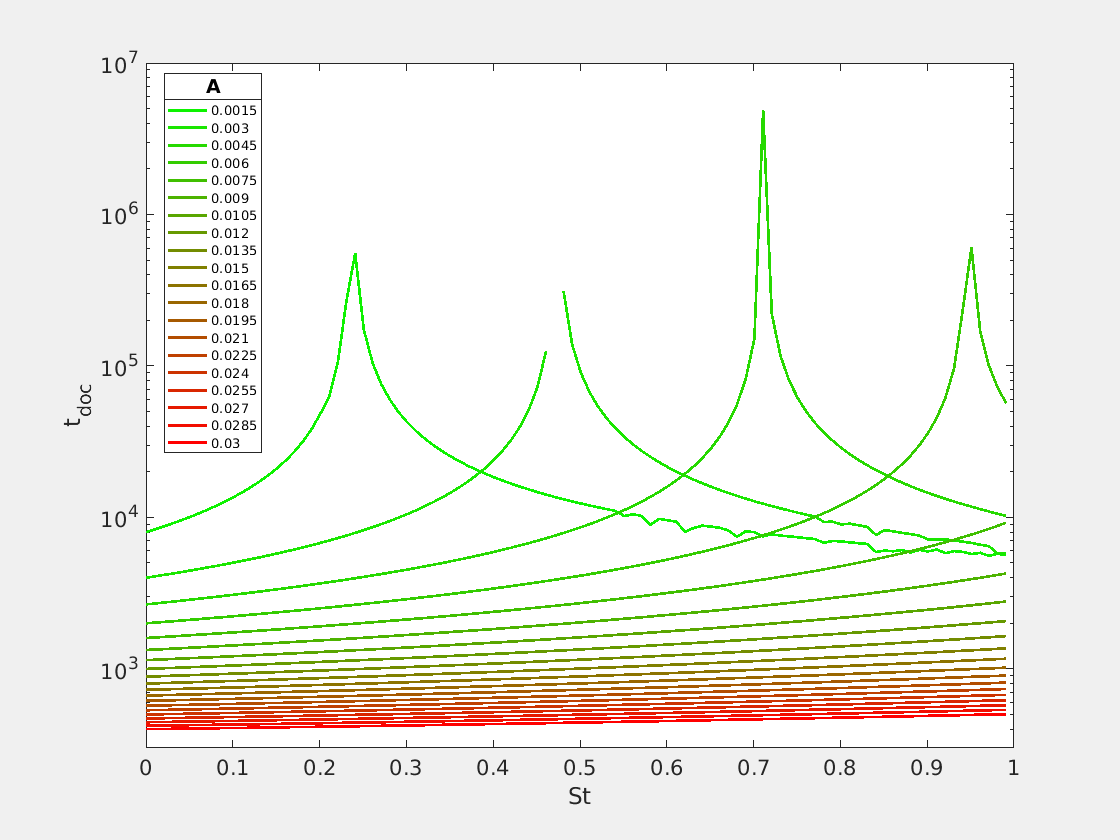
\includegraphics[width=30pc]{gfx/St_t_doc_A_full_eps000001.png}
\caption{Docking time calculated numerically with respect to  $St$ for a few chosen $A$ values, $\sigma=10^{-5}$.}
\label{fig:ch3_5}
\end{figure*}

\begin{figure*}
\centering
\noindent 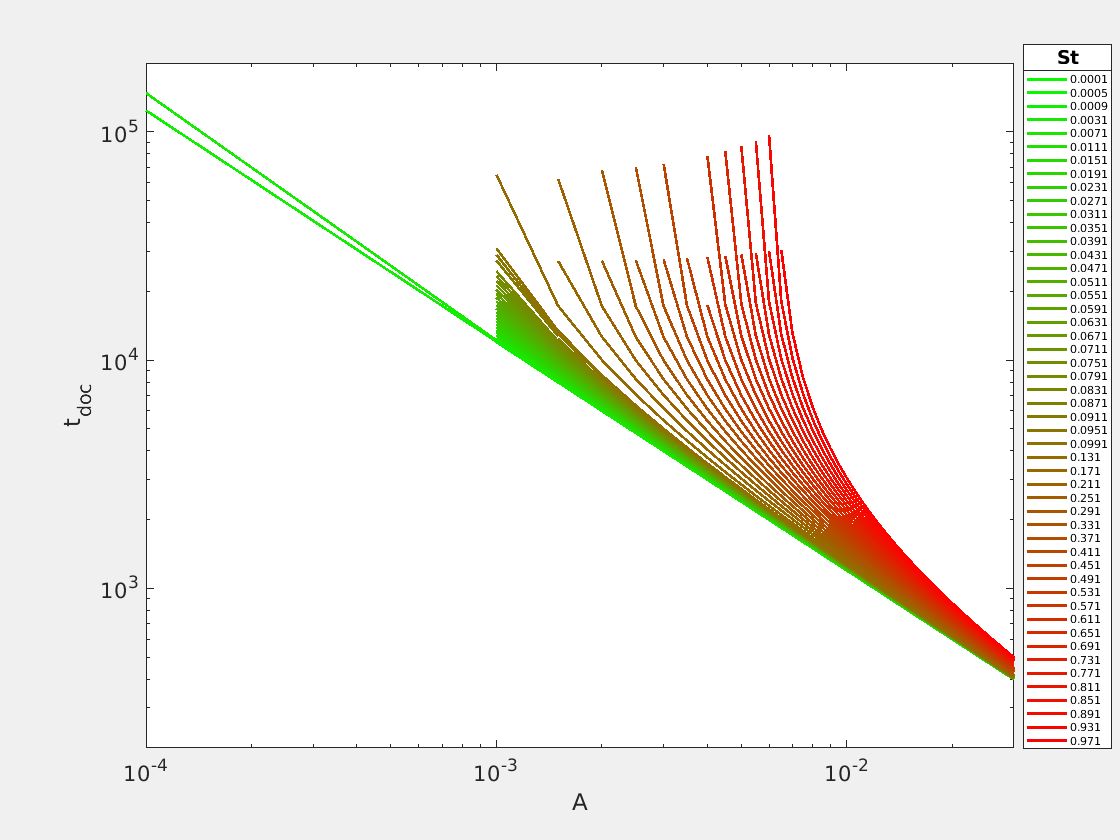
\includegraphics[width=30pc]{gfx/A_t_doc_St_part_right_eps000001.png}
\caption{Docking time calculated numerically with respect to $A$ for a few chosen $St$ values, for $A>St/16pi^2$, $\sigma=10^{-5}$.}
\label{fig:ch3_5a}
\end{figure*}

\begin{figure*}
\centering
\noindent 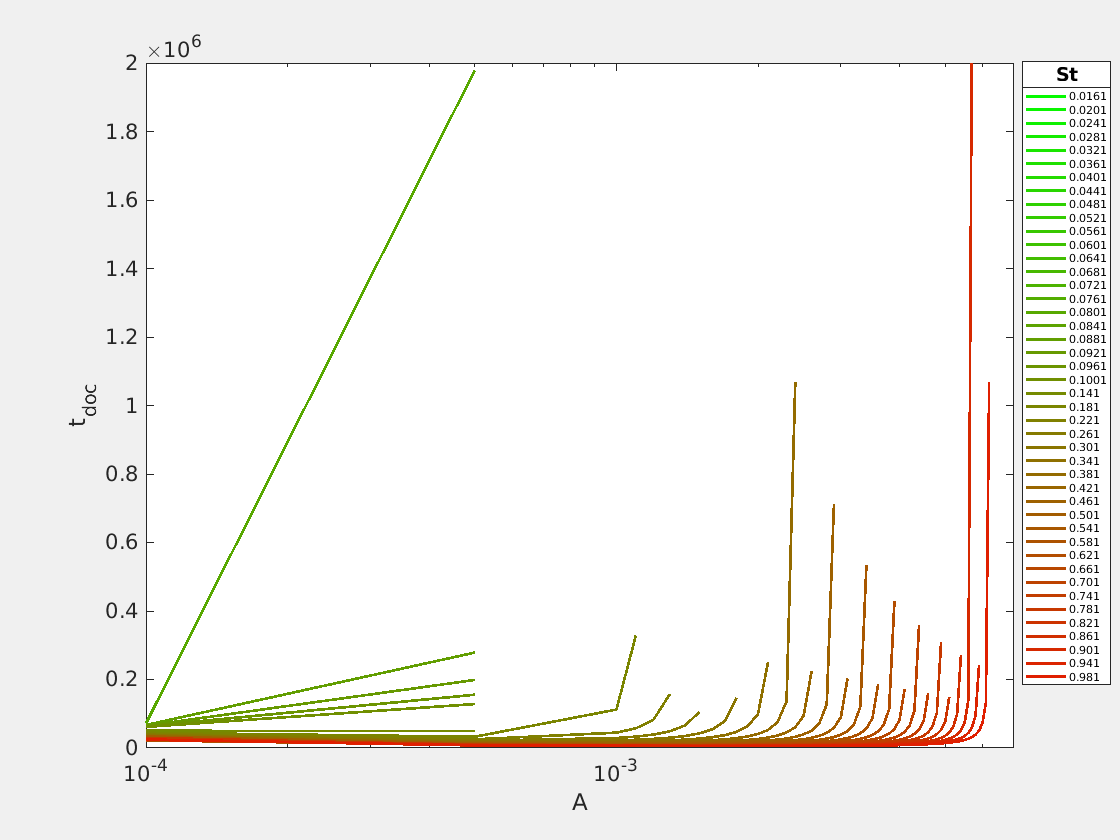
\includegraphics[width=30pc]{gfx/A_t_doc_St_part_left_logflat_eps000001.png}
\caption{Docking time calculated numerically with respect to $A$ for a few chosen $St$ values, for $A<St/16pi^2$, $eps=10^{-5}$.}
\label{fig:ch3_5b}
\end{figure*}

Since $\sigma$ in theory is infinitesimally small but the numerical calculation demands finite value, the sensitivity analysis was conducted below for $\sigma=10^{-n}, \ n=1,2,3,4,5$.\\
Dopisac, gdy juz cos wiecej bedzie wiadomo o samym czasie dokowania.
%\begin{figure*}
%\centering
%\noindent \includegraphics[width=30pc]{gfx/../gfx/.png}
%\caption{}
%\label{fig:ch3_5}
%\end{figure*}


\subsection{With gravity (inclined vortex)}
\noindent Nonparallel alignment of the gravity vector and vortex axis ($\theta \neq 0$) destroys the axial symmetry of the system and introduces the presence of other attractors, such as non-circular periodic orbit and multiple equilibrium points outside the axis.\\
 
For a nonzero $\theta$, every particle always has equilibrium points in 2D space. Position of these points in 2D space is determined by $S_v$ and $A$ and it can be uniquely determined by solving the equilibrium point equation:
\begin{equation}
 f_A(r^+) = S_v,
 \label{ch3:eq27}
\end{equation}
where function $f_A(r^+)$ is defined for each $A$:
\begin{equation}
f_A(r^+) = r^+ A \sqrt { 1 + \left( \frac{1-\exp \left(\frac{-r^{+ 2}}{2}\right)}{2\pi Ar^{+ 2}} \right)^2 }
 \label{ch3:eq28}
\end{equation}
and is called an equilibrium curve (see Fig.2 in \citet{Marcu1995}). Detailed analysis of this eqation's solutions is performed below.\\

\begin{table}
\small
\tabcolsep=0.2cm
\centering
\caption{Burgers vortex non-dimensional numbers}
\centering
\begin{tabular}{|l|c|}
\hline 
$A_{cr}$ & 0.02176 \\
\hline
$r_i$ & 2.1866\\
\hline
$S_{v i}$ & 0.0815\\
\hline
$r_s$ & 1.585201\\
\hline
$S_{v s}$ & 0.0718\\
\hline
\end{tabular}
\label{tab:ch3_2}
\end{table}

Equillibrium curves for a dozen of $A$ values are plotted in Fig. \ref{fig:ch3_6}. It is easy to find that $f_A(0)=0$ and $\lim_{r^+\to\infty} f_A(r^+)=\infty$. Moreover, there exists a critical value of nondimensional strain $A_{cr}$ for which bifurcation from one unique solution (for $A \geq A_{cr}$) to maximally three solutions (for $A<A_{cr}$) occurs. $A_{cr}$ corresponds to the equilibrium curve that has a horizontal slope at the inflection point. $A_{cr}$ value was estimated numerically (see the Table \ref{tab:ch3_2}). It is also easy to prove that the equillibrium curves asymptotically tend to the function $f_{A \rightarrow 0+}(r)=\left( 1-exp(-r^2/2)\right)/2\pi r$. This function, unlike equillibrium curves for $A \in (0,A_{cr})$ does not have a minimum.

\begin{figure*}
\centering
\noindent 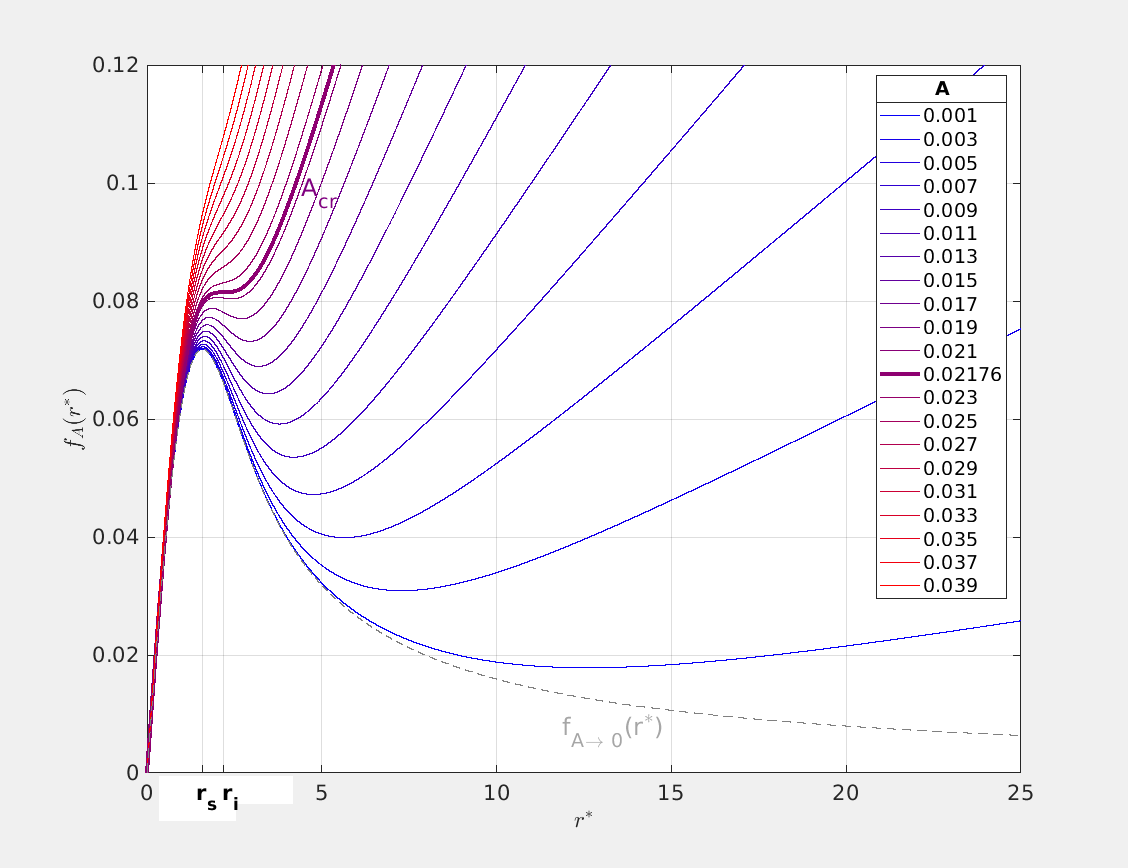
\includegraphics[width=30pc]{gfx/eq_curves.png}
\caption{Equillibrium curve plots for different $A$ values. $A_{cr}$, $r_s$, $r_i$ are defined in the text body. Gray dashed line shows an equillibrium curve which is an asymptotic limit of $A \rightarrow 0+$}
\label{fig:ch3_6}
\end{figure*}

For $A \geq A_{cr}$ the equilibrium curve is a monotonically increasing function of $r^+$ so there exists exactly one solution for every $S_v$ value.\\
For $A<A_{cr}$ the equilibrium curve always has one maximum at $r^+_{max}$ and one minimum at $r^+_{min}$. The inflection point of $A=A _{cr}$ equilibrium curve plot lies at $r_i$ and for $S_{v i}$ (numerical estimations in the Table \ref{tab:ch3_2}). It restricts values of $r^+_{max}$ from above and values of $r^+_{min}$ from below. Let's define:
\begin{align}
S_{v\ min}=f_A(r^+_{min}) \\
S_{v\ max}=f_A(r^+_{max})
\label{ch3:eq28b}
\end{align}
Consequently, for $S_v<S_{v\ min}$ and for $S_v>S_{v\ max}$, there is only one solution. For $S_v=S_{v\ min}$ and for $S_v=S_{v\ max}$, there are two solutions. For $S_{v\ min}<S_v<S_{v\ max}$, there are three solutions. All the conclusions are summarised in Table \ref{tab:ch3_2b}.

\begin{table}
\small
\tabcolsep=0.2cm
\caption{Existence and position of equilibrium points with respect to $A$ and $S_v$ parameters. $A_{cr}$, $r_s$, $r^+_{min}$, $S_{v\ min}$, $S_{v\ max}$ are defined in the text body.}
\centering
\begin{tabular}{|c|c|l|}
\hline
$A$ & $S_v$ & nr  of eq. points\\
\hline
$\geq A_{cr}$ & arbitrary & 1 \\
\hline
\multirow{3}{*}{$<A_{cr}$} & $<S_{v\ min}$ & 1 at $r^+_0 <r_s$ \\
\multirow{3}{*}{\ } & $[S_{v\ min},S_{v\ max}]$  & 2 or 3, I: $r^+_0\leq r^+_{max}<r_i$, II: $r^+_0 \in (r^+_{max},r^+_{min})$, III: $r^+_0>r^+_{min}$\\
\multirow{3}{*}{\ } & $>S_{v\ max}$  & 1 at $r^+_0>r^+_{min}>r_i$\\
\hline
\end{tabular}
\label{tab:ch3_2b}
\end{table}

Not only is the existence of the multiple solutions important but their stability as well. Let $r^+_0$ denote an arbitrary dimensionless solution of Eq. \ref{ch3:eq27}. The exact form of the stability condition of the solution $r^+_0$ is governed by the function $\phi(r^+_0)$ (as defined in \citet{Marcu1995}). The condition can take two different forms depending on the sign of this function:
\begin{equation}
\phi(r^+_0)=\frac{1}{(2 \pi)^2} \left[\frac{1-\exp(-r^{+ 2}_0/2)}{r^{+ 2}_0} \right] \left[\frac{1-\exp(-r^{+ 2}_0/2)}{r^{+ 2}_0}-\exp(-r^{+ 2}_0/2) \right].
\label{ch3:eq29}
\end{equation}
Plots of $\phi(r^+_0)$ and its square root are shown in Fig.\ref{fig:ch3_7}.

\begin{figure*}
\centering
\noindent 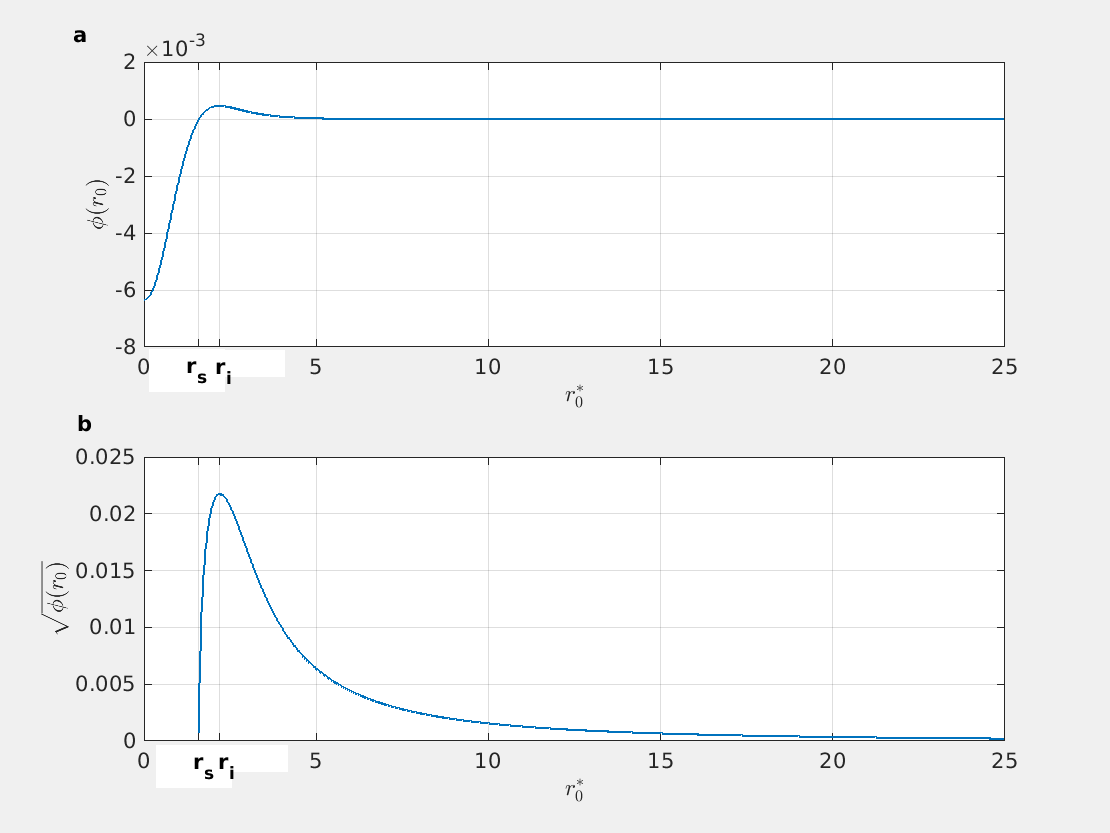
\includegraphics[width=30pc]{gfx/stability_functions.png}
\caption{Plot of the function $\phi(r^+_0)$ determining equillibrium point stability (a) and its square radius $\sqrt{\phi(r^+_0)}$ (b) with respect to equillibrium point radial position.}
\label{fig:ch3_7}
\end{figure*}

Function $\phi(r^+_0)$ has only one zero at $r_s$ (see Table \ref{tab:ch3_2}). For small radii, $r^+_0<r_s$, the equilibrium is a spiral/focus, and it is stable if:

\begin{equation}
St \leq \frac{A}{|{\phi(r^+_0)}|}.
\label{ch3:eq30}
\end{equation}

\noindent For greater radii, $r^+_0>r_s$, the equilibrium point is either a stable node or a saddle. The condition for stability depends explicitly only on $A$:
\begin{equation}
A \geq \sqrt{\phi(r^+_0)}.
\label{ch3:eq31}
\end{equation}
\\
Analysis of the equilibrium point stability conditions by \citet{Marcu1995} is expanded here with emphasis on the dependence on strain parameter $A$.  Because stability condition for larger radii $r^+_0 > r_s$ expressed by Eq.\ref{ch3:eq31} is independent of $St$, additional conclusions can be drawn. Numerical calculations lead to the result, that for every $A<A_{cr}$ there is:
\begin{equation}
\sqrt{\phi(r^+_{max}(A))}=\sqrt{\phi(r^+_{min}(A))}=A.
\label{ch3:eq32}
\end{equation}
In the range between maximum and minimum $r^+_0 \in (r^+_{max},r^+_{min})$ there is $\sqrt{\phi(r^+_0)} > \sqrt{\phi(r^+_{min}(A))}$, so the condition in Eq.\ref{ch3:eq31} is not satisfied and the points in this range are not stable. For $r^+_0 >r^+_{min}$ there is 
$\sqrt{\phi(r^+_0)} <\sqrt{\phi(r^+_{min}(A))}$, so the condition in Eq.\ref{ch3:eq31} is satisfied and the points in this range are stable.
In the case $A \geq A_{cr}$ the condition in Eq.\ref{ch3:eq31} is satisfied, because $A>\max_{r^+_0}\left( \sqrt{\varphi(r^+_0)}\right)=A_{cr}$. The unique solution is a stable node. These results are summarised in Table \ref{tab:ch3_3}.

\begin{table}
\small
\tabcolsep=0.2cm
\caption{Stability conditions of particle equilibrium points present in the Burgers vortex with respect to vortex strain parameter $A$ and dimensionless radial position $r^+$. $A_{cr}$, $\varphi(r^+)$, $r_s$, $r_i$, $r^+_{min}$ and $r^+_{max}$ are defined in the text body.}
\centering
\begin{tabular}{|l|c|c|c|c|}
\hline 
 & $ \leq r_s$ & $(r_s,r^+_{max})$ & $[r^+_{max}, r^+_{min})$ & $\geq r^+_{min}$ \\
\hline
$A < A_{cr}$ & \multirow{2}{*}{focus, unstable if $St>A/|\phi(r^+_0)|$} & stable node & saddle & stable node\\
\cline{3-5}
$A \geq A_{cr}$ &  \multirow{2}{*}{\ } & \multicolumn{3}{|c|}{stable node}\\
\hline
\end{tabular}
\label{tab:ch3_3}
\end{table}
 
The stability properties can be analysed with $S_v$ as a leading parameter too, in contrast to equilibrium curve viewpoint. Figure \ref{fig:ch3_8} presents equilibrium point $r^+_0$ plots versus $A$. Line colors refer to various $S_v$ parameters. Continous line represents stable point, dashed - unstable. Three colored regions in the background mark three stability domains: light gray corresponds to condition in Eq.\ref{ch3:eq31} satisfied (a stable node), light green to the same condition not satisfied (a saddle), light red points to the focus region $r^+_0<r_s$. Stability of the focus is governed by Eq.\ref{ch3:eq30}, so $St$ must be considered as well. An example of stability properties in the region $r^+_0<r_s$ is shown by the cross signs - they represent the example of unstable focii for $St=0.5$. $r_s$, $r_i$ and $A_{cr}$ are marked on the axes for reference.

\begin{figure*}
\centering
\noindent 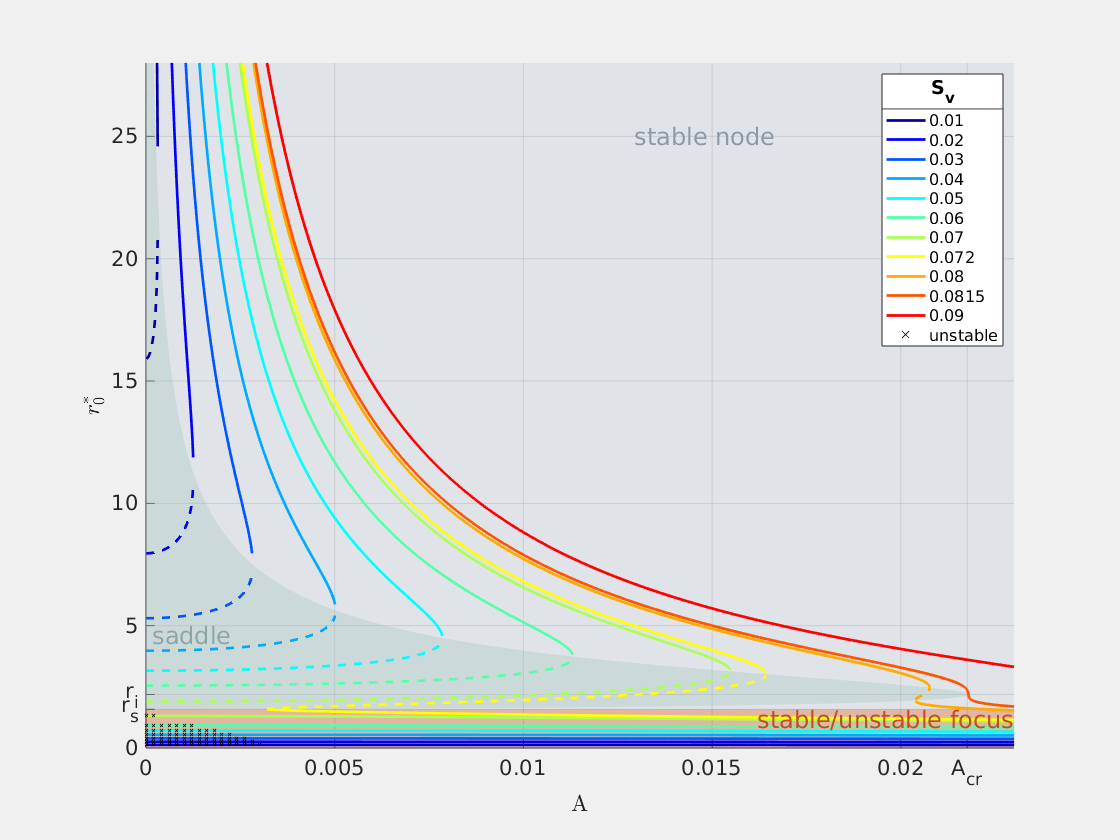
\includegraphics[width=30pc]{gfx/r0_vs_A_plus_stability.png}
\caption{Equilibrium point $r^+_0$ position versus $A$. Line colors refer to various $S_v$ parameters, continous line - to stable point, dashed line - to unstable. The colored regions in the background mark various stability subdomains: light gray - a stable node, light green - a saddle, light red - a focus. Crosses show example of unstable focii in the light red region for the case of $St=0.5$.}
\label{fig:ch3_8}
\end{figure*}

In Fig. \ref{fig:ch3_8}, the following conclusions about stability can be drawn.  For $S_v<S_{v s}$ there is at least one focus near the axis, at $r^+_0<r_s$, stable or unstable. When $A \geq A_{cr}$ it is unique, when $A<A_{cr}$ it can be accompied by a saddle and a stable node or a stable node itself. For $S_v \in (S_{v s},S_{v i})$ and when $A<A_{cr}$ there is at least the stable node far from the axis. In addition there can be the saddle and the stable node near the axis, the saddle and the focus or the focus itself. When $A \geq A_{cr}$ there is only one point near the axis and it is either a focus or a stable node. For $S_{v i}$ there is bifurcation from three possible solutions to just one. When $A<A_{cr}$ the one is a unique stable node far from the axis, when $A \geq A_{cr}$ it is a unique stable node at arbitrary position or a focus near the axis.\\

\begin{figure*}
\centering
\noindent 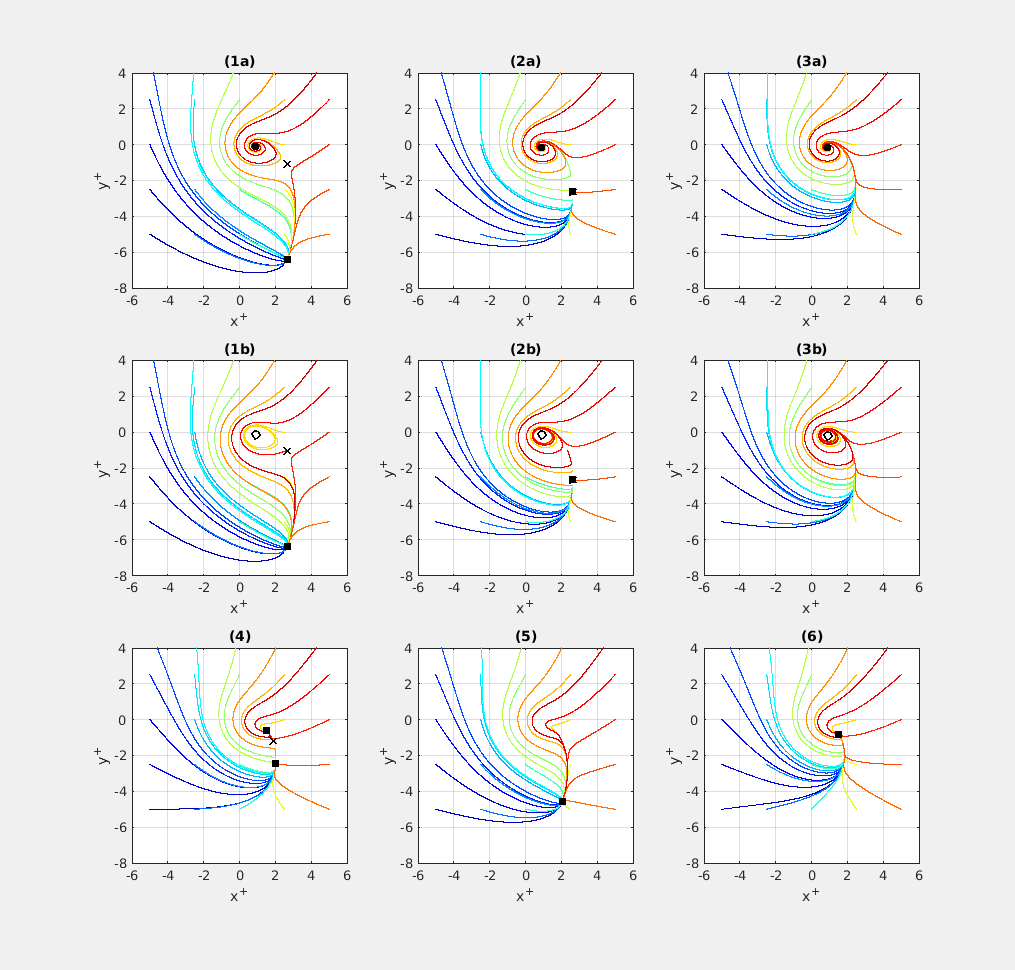
\includegraphics[width=30pc]{gfx/scenarios_9p_T500_D5_N5.png}
\caption{Particle trajectory plots for various sets of $(A,Sv,St)$ parameters. In each figure 25 particles are initialised at regular grid with zero velocity. Line colors vary in order to improve clarity. Scattered points represent equilibrium points position, their shape refer to their dynamical type: $\times$ - a saddle, $\circ$ - a focus (filled means stable), $\square$ - stable node. "a" and "b" types present the same $(A,Sv)$ sets, but with different $St$ determining stability of the focus ("a" - stable, "b" - unstable).}
\label{fig:ch3_9}
\end{figure*}

The combination of multiple point existence conditions with stability conditions creates a variety of single particle motion scenarios. Some of them were shown in Fig.4-9 in \citet{Marcu1995}. Fig. \ref{fig:ch3_9} here illustrates all nine of these combinations, by showing trajectory plots of particles initially positioned on the chosen grid with zero velocity. Trajectories were calculated numerically for representative sets of parameters. Different line colors are only intended to improve the plot clarity. Singular markers indicate the position of the equilibrium points, while their shape - their dynamic character. Tab.\ref{tab:ch3_4} summarises the analysis by showing $A$ and $Sv$ parameter ranges with relevant scenarios, as pictured in Fig. \ref{fig:ch3_9}.

\begin{table}
\small
\tabcolsep=0.2cm
\caption{Single particle motion scenarios with respect to $A$ and $S_v$ parameters. Numbers refer to Fig.\ref{fig:ch3_9}}.
\centering
\begin{tabular}{|c|c|c|}
\hline 
 & $A < A_{cr}$ & $A \geq A_{cr}$\\
\hline
$S_v<S_{v s}$ &(1) (2) (3) & (3)\\
\hline
$[S_{v s},S_{v i}]$ & (1) (2) (4) (5)& (3) (6)\\
\hline
$S_v>S_{v i}$ & (5) & (3) (5) (6)\\
\hline
\end{tabular}
\label{tab:ch3_4}
\end{table}

These scenarios are used later to carry out a search for vortex model parameter values that produce a void. 
\\
Dodac cos tutaj o tej publikacji Sapsin And Haler 2010 o przyciaganiu czastek inercyjnych przez powolne rozmaitosci.

\section{Time scales of single particle motion}
We were able to find approximate relations of a few timescales for single particle motion in Burgers vortex: exit time $\tau_{ex}$, connected to timescale of motion along the axis $\tau_z$, no-gravity orbit rotation time $\tau_{orb}$ and no-gravity axis docking time $\tau_{d1}$. For ease of reference, these approximations are summarised in Table \ref{tab:ch3_5}. Several conclusions about three dimensional particle motion can be drawn from the comparison of the separately derived time scales:
\begin{enumerate}
\item $\tau_{d1}$ and $\tau_z$ are approximately independent of particle radius $R$ and vortex strain $A$.
\item $\tau_{orb}<<\tau_z$
\item $\tau_{orb}<<\tau_{ex}$ as long as the logarithmic part in Eq.\ref{ch3:eq14} is not significantly smaller than 1. It means that particle starting far from vortex "lids' is able to swirl around the vortex axis for significant amount of time before being expelled by motion along vortex axis.
\item $\frac{\tau_{ex}}{\tau_{d1}}=4 \log L(a_1,a_2)$, which implies that axis docking time and exit time are of the same order as long as $\log L(a_1,a_2)$ is close to $1/4$. It means that particle starting position and vortex length determines the fact if particle is able to approach its stable point on vortex axis befor being expelled.
\end{enumerate} 


\begin{table}
\small
\tabcolsep=0.2cm
\caption{Tabeleczka}.
\centering
\begin{tabular}{|c|c|c|}
\hline 
 &  & \\
\\
\hline
\end{tabular}
\label{tab:ch3_5}
\end{table}

Tu nastapi jakies podsumowanie rozdzialu.
\end{document}